\documentclass{sig-alternate}
% graphic declaration
\usepackage{graphicx}
\usepackage{listings}
\usepackage[english]{babel}
\usepackage{float}
\usepackage{color}
\usepackage{caption}
\usepackage{indentfirst}
\usepackage{amsmath}
\usepackage{fancybox}
\usepackage{algorithm}
\usepackage{algpseudocode}
\usepackage{multicol}
\usepackage{balance}
%\usepackage{svg}
\usepackage{pdfpages}

\definecolor{dkgreen}{rgb}{0,0.6,0}
\definecolor{gray}{rgb}{0.5,0.5,0.5}
\definecolor{mauve}{rgb}{0.58,0,0.82}


\def\denseitems
{
  \itemsep1pt plus1pt minus1pt
  \parsep0pt plus0pt
  \parskip0pt\topsep0pt
}
%\iffalse
%\lstset{frame=tb,
  %language=Java,
  %aboveskip=3mm,
  %belowskip=3mm,
  %showstringspaces=false,
  %columns=flexible,
  %basicstyle={\footnotesize\ttfamily},
  %numbers=none,
  %numberstyle=\tiny\color{gray},
  %keywordstyle=\color{blue},
  %commentstyle=\color{dkgreen},
  %stringstyle=\color{mauve},
  %breaklines=true,
  %breakatwhitespace=true,
  %tabsize=3
%}
%\fi

\lstset{%
  xleftmargin=0pt,	
  belowcaptionskip=\bigskipamount,
  captionpos=b,
  escapeinside={*'}{'*},
  language=Java,
  tabsize=2,
  emphstyle={\bf},
  commentstyle=\it,
  stringstyle=\mdseries\ttfamily,
  showspaces=false,
  keywordstyle=\bfseries,
  morekeywords={then,end,String,Class,Object},
  columns=flexible,
  basicstyle=\footnotesize\ttfamily,
  showstringspaces=false,
  morecomment=[l]\%,
}

\graphicspath{ {data/} }

\begin{document}

\setcopyright{acmcopyright}
\conferenceinfo{DEBS '16}{June 20--24, 2016, Irvine, CA, USA}
\acmPrice{\$15.00}
%\doi{}

\makeatletter
\renewcommand{\@maketitle}{
\newpage
 \null
 \vskip 2em%
 \begin{center}%
	{\ttlfnt \@title\par}
	\vskip 10em                % Vertical space after title.
 \end{center}%
 \par} \makeatother

%
% paper title
% Titles are generally capitalized except for words such as a, an, and, as,
% at, but, by, for, in, nor, of, on, or, the, to and up, which are usually
% not capitalized unless they are the first or last word of the title.
% Linebreaks \\ can be used within to get better formatting as desired.
% Do not put math or special symbols in the title.
%\title{Expanding Limited Mobile Resources for Performance, Energy-Efficiency, and Privacy}
%\title{Extending Resource-Constrained Mobile Devices for Performance, Energy-Efficiency, and Privacy}
\title{Utilizing Nearby Distributed Computing Resources for Resource-Limited Mobile Devices}
%Resource-Constrained Mobile Devices}

%%%N-REX (Nearby-Remote Executor similar to T-Rex)

% author names and affiliations
% use a multiple column layout for up to three different
% affiliations
\numberofauthors{2}
\author{
\alignauthor Le Dinh Minh \\
\affaddr{Department of Computer Science} \\
\affaddr{Utah State University} \\
\email{minh.le@aggiemail.usu.edu}
\alignauthor Young-Woo Kwon \\
\affaddr{Department of Computer Science} \\
\affaddr{Utah State University} \\
\email{young.kwon@usu.edu}
}

% make the title area
\maketitle

\begin{abstract}
For the last decade, mobile devices have been significantly developed with powerful hardware facilities such as multicore CPUs, large and fast memory, fast network and high-resolution displays. As a result, mobile applications deliver increasingly complex functionality from the recent past. Furthermore, rapid growth in application functionality requires ever greater hardware capability. Thus ensuring the quality of service in resources-limited execution environments remains a major challenge of mobile software development. To reduce execution time and save battery power, some functionality of mobile applications is often executed on a remote server. However, such an optimization mechanism (i.e., computational offloading) has only received much attention in the research literature due to difficult implementation, limited applicability, the cost of the cloud, etc. In this paper, we present a novel distribution infrastructure that executes any functionality at a powerful remote server or nearby mobile devices using two distributed execution models---client/server and peer to peer. By means of a simple programming model, the programmer can easily adopt two distributed execution models in their applications. Our benchmarks and case studies demonstrate that the new distribution infrastructure can increase both performance and energy efficiency of mobile applications as well as introduce the new feature (i.e., sensors) to the existing mobile devices.
\end{abstract}

\begin{CCSXML}
<ccs2012>
<concept>
<concept_id>10010520.10010521.10010537</concept_id>
<concept_desc>Computer systems organization~Distributed architectures</concept_desc>
<concept_significance>100</concept_significance>
</concept>
<concept>
<concept_id>10010520.10010521.10010537.10010540</concept_id>
<concept_desc>Computer systems organization~Peer-to-peer architectures</concept_desc>
<concept_significance>100</concept_significance>
</concept>
</ccs2012>
\end{CCSXML}

\ccsdesc[100]{Computer systems organization~Distributed architectures}
\ccsdesc[100]{Computer systems organization~Peer-to-peer architectures}
\terms{Design}

\printccsdesc
\keywords{Mobile Application, Remote Execution, Offloading, Peer to Peer, Runtime System}

\section{Introduction}
Mobile devices have been evolving at the lightning pace with powerful hardware facilities such as multicore CPUs, large and fast memory, fast network and high-resolution displays. Due to the significant development of mobile hardware, today's mobile applications are becoming more complex with an increasingly feature-rich nature. As a result, mobile devices often overtake the personal computer as a primary means of accessing computing resource. However, the resource demands (e.g., computation, memory, battery, etc.) of mobile applications often outstrip the hardware capacities of mobile devices. A particularly popular technique to extend limited mobile hardware is \emph{computational offloading}---executing CPU-intensive functionality at a powerful cloud-based server, thereby improving both performance and energy efficiency. 

Although computational offloading has been widely enjoyed in the research literature as an optimization mechanism that can utilize remote CPU resources, a majority of feature-rich mobile applications still suffer from resource constraints to provide quality user experiences. In addition, because computational offloading mechanisms have been developed by leveraging cloud computing technologies, in spite of their significant advantages, the high operational cost of cloud infrastructures and the implementation difficulties of computational offloading have deterred programmers from actively applying computational offloading in their mobile applications. In particular, performance or energy benefits gained through computational offloading would be considerably low when comparing to the operational costs of the cloud-based offloading server. Moreover, mobile devices can only execute computation-intensive functionality by accessing the cloud-based server. Finally, implementing effective computational offloading optimizations often requires highly experienced programming skills and efforts \cite{kwon+:mobilesoft2015}.

Nevertheless, computational offloading is still considered an important optimization mechanism for mobile applications as one of distributed execution models. To optimize mobile applications' performances and extend their hardware capacities through distributed executions, we solve the following research problems: (1) how can mobile applications utilize remote computing resources at low cost? (2) how can the application programmer express the desired mobile hardware resources? (3) how can mobile devices allow using their resources without affecting the existing applications' executions? Solving these problems requires innovations in programming models and middleware design spaces. 

In this paper, we present a novel distributed execution model that not only optimizes mobile application's executions in terms of performance and energy efficiency but also extends mobile device's hardware capability. In other words, mobile devices will be able to add virtually more hardware resources including computation, networking, memory, and sensors to the existing hardware setups. Our approach is realized as the following major technical solutions: (1) a straight programming model that enables the programmer to write any execution task and (2) a runtime system that determines an execution strategy and distributes the requested execution task over the nearby or remote network. Our runtime system employs a dynamic, adaptive mechanism to determine the best distribution and execution strategy under different execution environments including diverse network conditions and heterogeneous mobile devices.

The experiments in three case studies have demonstrated the effectiveness of our approach, to extend limited mobile hardware resources, thereby improving performance and energy efficiency as well as bringing new hardware capabilities. By presenting our approach, this paper makes the following technical contributions:
\begin{itemize} \denseitems
	\item \textbf{Simple programming model:} We provide simple APIs for programmers to easily deploy distributed mobile applications to take full advantage of external remote resources using our distributed execution model.
	\item \textbf{Lightweight runtime system:} Our runtime system efficiently distributes executions to available peers or offloading server, based on a peer selection algorithm. 	
	\item \textbf{A proof of concept infrastructure implementation:} Through three case studies, our system demonstrates how mobile hardware resources can be effectively shared.
\end{itemize}

%should go to the later part
%No internet connections are required, and it will help the owner to connect to the devices within a closed distance. By establishing connection between the two devices to form a pair, Wi-Fi Direct can provide the simple way to dynamically initiate a peer-to-peer network. Available on Android devices from version 4.0 (which more than 96\% of devices are using these days), as well as a number of Intel-featured laptops and game consoles, there is the high possibility of discovering the other mobile devices at anywhere.

%Job2P provides a simple and straightforward API interface to get rid of sophistication of network implementation, letting developers easily create their distributed mobile applications with capability of forming closed range network. In term of workload distribution, Job2P splits task and resource into the smaller units called jobs, and dispatch to the peers. To distributed jobs equitably among the peers, a decision making module is added to decide the amount of resource the peer has to handle bases on its percentage of availability. Moreover, our APIs can handle fault tolerant for network malfunctions.

The rest of this paper is structured as follows. Section \ref{sec:background} introduces a technological background for the main technologies used in this work. Section \ref{sec:approach} details our technical approach and Section \ref{sec:eval} discuss how we evaluated our approach. Section \ref{sec:related} compares our approach to the related state of the art. Section \ref{sec:conc} concludes this paper.
 
\section{Technical Background}
\label{sec:background}
In this section, we present the major technologies used in this paper including remote execution (remote procedure call, computation offloading, and mobile agent), peer-to-peer network, and middleware. We will describe them in the following subsections.

\subsection{Remote Execution}   
\textbf{Remote Procedure Call (RPC).} RPC has become the basis for modern middleware systems. In this model, each call to a remote object is sent from the client to the server and then the results are returned to the client. In distributed/mobile computing, the RPC model has been widely used for performance and energy-efficiency optimizations. In this paper, our approach heavily relies on the RPC model for discovering nearby devices, dispatching a job, and monitoring peer status.

\textbf{Computation Offloading.} Computation Offloading---executing computation-intensive functionality and receiving a result only---has become a popular optimization technique for mobile applications \cite{maui,chun+:eurosys11,kwon+:icsm13,wen2012energy}. It leverages the resources of cloud-based remote servers to execute portions of a mobile application's functionality. By executing some of the application's functionality in the cloud, offloading reduces the amount of energy consumed by the mobile device, thus saving its battery power. An additional benefit of computation offloading is improved performance efficiency, as cloud servers have hardware resource more powerful that those available on mobile devices. This technique is used as one of the distributed execution models in this paper.

\textbf{Mobile Agent.} Mobile agent was introduced to move computer programs within distributed systems and act on behalf of the user. The programs can be executed near the data, thereby reducing data transmission time and improving the overall performance \cite{peine+:ma99}. The concept of the mobile agent have been applied to the grid computing to allocate remote computing resources so that users can execute their jobs on the remote machines \cite{fukuda+:ma_grid03}. By embracing the concept of mobile agent, our approach allows resource-limited mobile devices to utilize nearby computing resources for improving performance and energy efficiency as well as introducing a new hardware feature.

\subsection{Peer-to-Peer Network and WiFi Direct}
WiFi Direct \cite{alliance2010wi} is a new peer to peer standard built on top of the IEEE 802.11 to provide direct connections between WiFi devices without an Internet connection. Over a WiFi network, a WiFi device can discover and connect to any types of WiFi devices without special configurations or setups. Once a connection is established, WiFi devices can communicate with each other as a client or an access point. WiFi Direct has been widely used to transfer content or share applications between mobile devices. Recently in Android, WiFi Direct has been available from Android 4.0 APIs. In this paper, our approach uses Android WiFi Direct \cite{wifi:p2p} to utilize nearby computing resources without an Internet connection or wireless access point (AP). Even though the discovery operation of WiFi Direct is costly \cite{trifunovic2013slicing}, our approach is still efficient for CPU-intensive executions and sharing hardware resources. 

\subsection{Middleware}
Middleware systems provide programming and runtime support to coordinates the execution of multiple remote processes. By eliminating the need for low-level network programming (e.g., managing sockets, marshaling/unmarshaling data, keeping track of processes), middleware offers convenient building blocks for constructing distributed systems. Moreover, several middleware infrastructures provide a programming model as well as advanced functionality to improve performance- and energy-efficiency \cite{kwon+:mobilesoft2015}. Thus, our approach uses these features from mainstream middleware mechanisms for distributed execution as building blocks. 

%In our prior work \cite{kwon+:mobilesoft2015}, we introduced a programming model and a middleware architecture for performance and energy optimization. The runtime system developed in this paper is derived from our prior middleware design.


%other name?
\section{Our Approach}
\label{sec:approach}
In this section, we present our approach, a distributed mobile execution model that can expand the resource capacities of mobile devices. We start by giving an overview of the approach and then describe its major parts.

\begin{figure}
	\centering	
		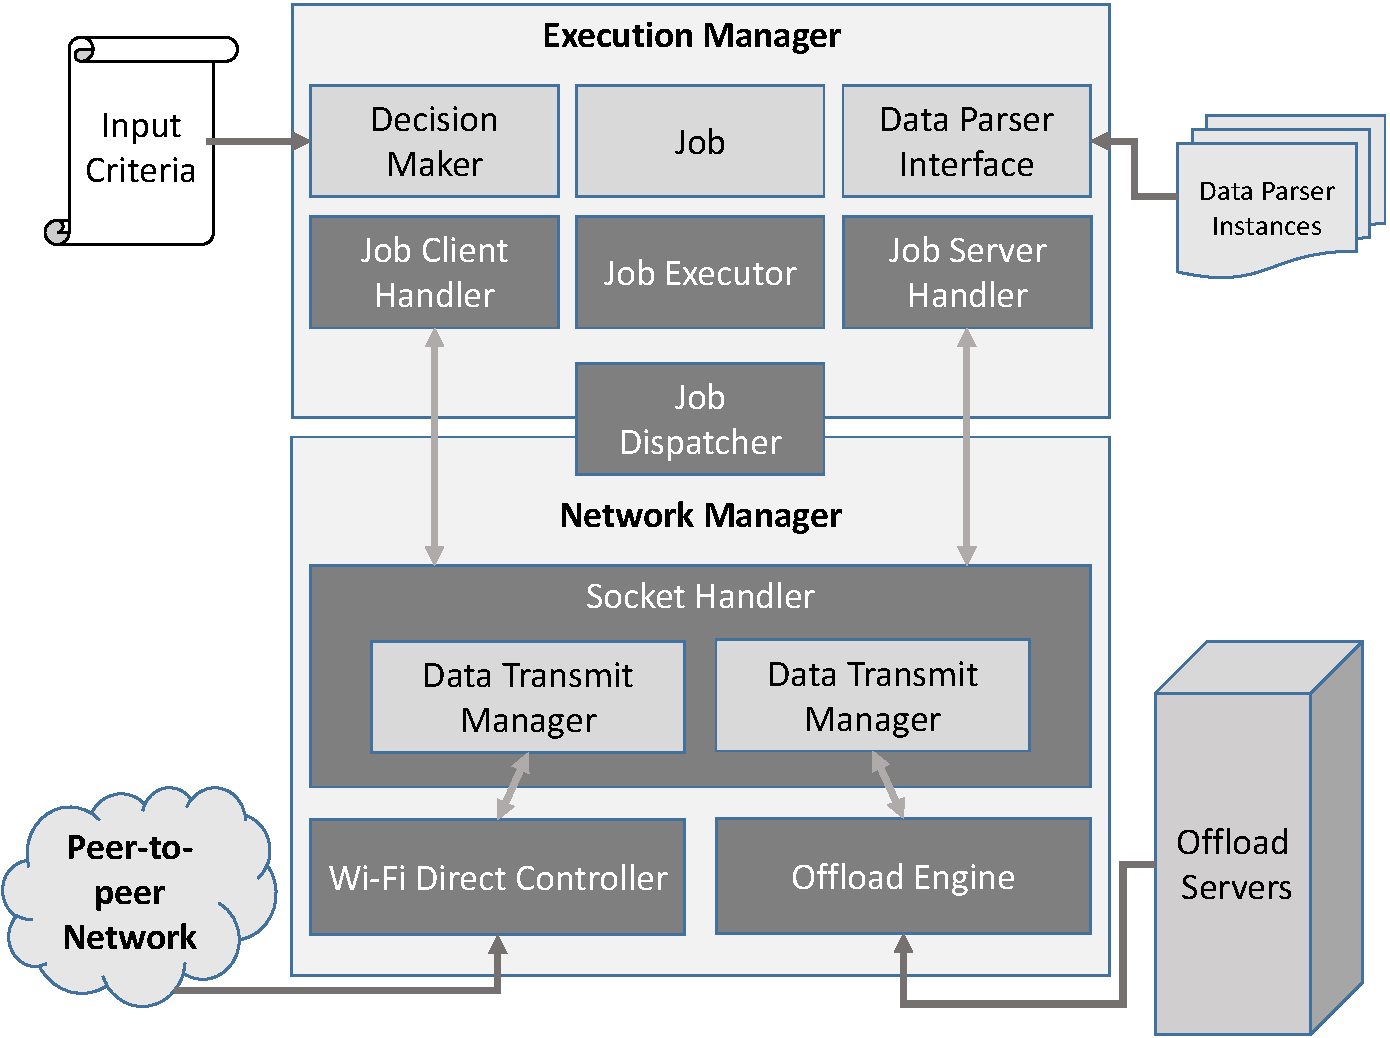
\includegraphics[width=.98\linewidth]{data/jobShareArch.pdf}	
	\caption{The overall system design.}
	\label{fig:architecture}
\end{figure}


\subsection{Approach Overview}
Figure \ref{fig:architecture} shows the overall system design that comprises two main components: (1) \emph{Execution Manager} determines appropriate distribution units and targets and then steers job executions and (2) \emph{Network Manager} discovers available mobile devices, checks the availability of the registered cloud-based remote servers, and then establishes a network connection for data transmissions. For the optimal execution result, \emph{Execution Manager} keeps track of current execution environments such as network conditions (e.g., delay, bandwidth) and system status (e.g., resource usage including CPU, memory). Finally, we offer a simple programming model that hides complex implementation details such as distributing a job and steering its execution, so that the programmer can introduce distribution to his/her program as well as extending the provided runtime system.

\emph{Execution Manager} selects the best available distribution targets, assigns a job to nearby peers or an offloading server, and steers its execution. Since we provide a simple programming model to enable the programmer to execute any kinds of jobs without the ad-hoc modification of the runtime system, the programmer first must implement both the \texttt{Job} and \texttt{DataParser} class, which will be discussed in Section \ref{prog_model}. Then, the module selects a number of favorable peers based on the current runtime condition and peers' system status if peer to peer execution is more beneficial than executing on an offloading server. Once all the distribution targets are determined, the job is dispatched with the appropriate amount of data. On the caller side, \emph{Execution Manager} dynamically loads the \texttt{Job} class and executes it. Finally, the execution result is sent back to the caller and is naturally migrated with other results by \texttt{DataParser}.

\begin{figure} [!tbh]
	\centering
	\resizebox{.95\linewidth}{!}{
		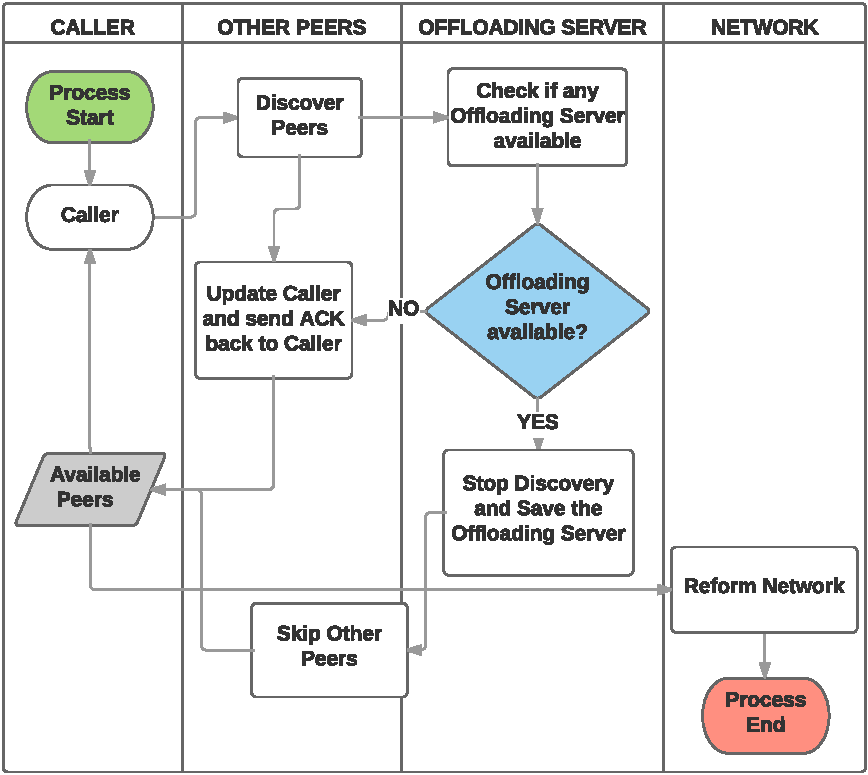
\includegraphics{data/discoverPeers.pdf}
	}
	\caption{Establishing a network connection between devices}
	\label{fig:forming}
\end{figure}

\emph{Network Manager} opens a communication channel, monitors peers' execution status, and handles faults. First, the module discovers all available nearby devices through WiFi Direct and check the availability of a cloud-based offloading server. By providing transparent operations between the offloading server and nearby mobile devices, our approach allows the programmer only to focus on his/her business logic. The \emph{Network Manager} sends a very short status inquiry message to the discovered devices and measures runtime conditions such as end-to-end latency, etc, and then each peer sends its information in a JSON format (see \ref{ss_dfp}). Next, \emph{Execution Manager} can determine the best execution strategy (e.g., peer-to-peer execution vs. cloud offloading, the optimal number of peers, the amount of data to be assigned to each peer, etc.). Once the available device list is determined, a communication channel is organized as described in Figure \ref{fig:forming}. Finally, the module keeps monitoring peers' execution status through WiFi Direct's exception handling mechanism, so that if there is any fault during the execution, \emph{Network Manager} catches the exception and then \emph{Execution Manager} immediately restarts the failed job locally. In addition to the exception handling mechanism, the module uses checksum to verify data integrity.

Our approach mainly comprises two parts: a programming model and runtime system. We describe these parts in turn next.

\subsection{Programming Model} \label{prog_model}
In this section, we discuss a programming model provided for application programmers. As described in Listing \ref{code:job_def}, the \texttt{Job} abstract class should be extended by the programmer to specify which functionality needs to be executed remotely. 

\subsubsection{Defining a Job}
Job implementation is the prerequisite work to determine what to execute on the remote device and how to cast and manipulate data from the abstract object. First, programmers should extend the \texttt{Job} class as well as overriding its \texttt{exec()} method. The \texttt{Job} class defines how the distributed job should be executed. 


\begin{figure} [!tbh]
\noindent \shadowbox{%
\begin{minipage}{.95\linewidth}
	\begin{lstlisting}
	public abstract class Job {
	  public abstract Object exec(Object param); }
	\end{lstlisting}	
\end{minipage}}	
\noindent \shadowbox{%
\begin{minipage}{.94\linewidth}
  \begin{lstlisting}
public interface DataParser {  
  public Class getDataClass();
  public byte[] parseObjectToBytes(dataObject);
  public Object parseBytesToObject(byteArray);
  public Object getSinglePart(..., 
						numOfParts, sOffset, eOffset);    
  public Object createPlaceholder(jsonMetadata);
  public Object copyPartToPlaceholder(... 
						partDataObject, sOffset, eOffset);
  public void destroy(dataObject);  }
  \end{lstlisting}	
\end{minipage}
}	
\captionof{lstlisting}{Programming model (APIs).}
\label{code:job_def}
\end{figure}

\subsubsection{Processing Application-Specific Data} \label{data_parser}
The \texttt{DataParser} interface defines how data should be processed (e.g., read/write), partitioned, and merged. \texttt{DataParser} described in Listing \ref{code:job_def} has the following methods:
\begin{itemize} \denseitems
	\item \texttt{getDataClass()} returns the data type.
	\item \texttt{parseObjectToBytes(object)} serializes an object to a binary array. 
	\item \texttt{parseBytesToObject(byte[])} deserializes a binary array back to an object.
	\item \texttt{getSinglePart()} partitions data based on number of parts (\texttt{numOfParts}) and its \texttt{index}. Listing \ref{code:get_single_part} shows an example to partition a bitmap image file. 
	\item \texttt{copyPartToPlaceholder()} merges partitioned and processed when a result is returned back to a caller from peers.
\end{itemize}

Through three case studies (Section \ref{sec:eval}), we evaluated our programming model (i.e., bitmap image processing, internet sharing, and GPS accessing). We will discuss how to use these APIs in Section \ref{sec:apiusage}.


\subsection{Runtime System} \label{scheduling}
In this section, we discuss about (1) how to discover available peers and exchange peers' information, (2) how to select appropriate peers, and (3) how to partition data to be sent to the selected peers. 
%These problems will be addressed by our \texttt{DecisionMaker} module.

\subsubsection{Discovering Available Peers}\label{ss_dfp}
During the initialization phase, our runtime system first bootstraps the peer discovery process by sending a broadcast messages to nearby peers for collecting peers' information. Once a runtime system receives a status inquiry message from nearby devices, it immediately sends a response message in a JSON format as shown in Listing \ref{code:jsonResponse}. While most fields are self-explanatory, \texttt{RL} (Responsiveness Level) is a parameter that represents how favorable the selected peer is to execute the requested job. We will further discuss this parameter in Section \ref{ss_ers}. The \texttt{availability} parameter is determined by the current level of battery usage. By default, if a device's battery level is higher than 80\%, its value is set to \texttt{on}. Otherwise, it is \texttt{off}. However user can override this threshold by updating the \texttt{availability-threshold} property in the configuration file\footnote{We currently use a simple key-value configuration file to specify user-specific preferences.} before the runtime system starts. 

\begin{figure} [!tbh]
\noindent \shadowbox{
\begin{minipage}{.95\linewidth}
\begin{lstlisting}
JSON : DeviceInfo {
	"availability": Boolean, "gps": Boolean,
	"network": ["low"|"high"|"off"], "RL": Double}
\end{lstlisting}			
\end{minipage}}	
%\\
%\noindent \shadowbox{%
%\begin{minipage}{243pt}	
%\begin{lstlisting}
%JSON : Condition {"RL": "max", "gps": "on"}
%\end{lstlisting}\end{minipage}}	
\captionof{lstlisting}{JSON response message.}
\label{code:jsonResponse}
\end{figure}

%\begin{figure}
%\noindent \shadowbox{
%\begin{minipage}{240pt}
%\begin{lstlisting}
%JSON : DeviceInfo {
  %"device": "LG-Volt", 
	%"RL": 24.83,
  %"availability": "off", 
	%"network": "low", 
	%"gps": "on",	
  %"cpu": {"usage": "0.3", "speed": "1.3", "cores": 4},
  %"memory": {"usage": "0.5", "total": 2},
  %"battery": {"usage": 0.85, "total": 2800}}
%\end{lstlisting}			
%\end{minipage}}	\\
%\noindent \shadowbox{%
%\begin{minipage}{243pt}	
%\begin{lstlisting}
%JSON : Condition {"RL": "max", "gps": "on"}
%\end{lstlisting}\end{minipage}}	
%
%\captionof{lstlisting}{JSON response format and initiative condition.}
%\label{code:jsonResponse}
%
%\end{figure}

%Where \texttt{device} parameter can be either device name (if it is a peer) or \texttt{Hostname/IP} (if it is offloading server), \texttt{RL} is the device's Response Level (Estimation of $RL$ will be covered in Sub section \ref{ss_ers}), \texttt{availability} indicates whether the device is ready for the job. \texttt{network} gives the Internet connection status, which can be either \texttt{high}, \texttt{low} or \texttt{off} (no connections), \texttt{gps} shows GPS status which can be either \texttt{on} or \texttt{off}. Finally \texttt{cpu}, \texttt{memory} and \texttt{battery} are the status of the essential resources at the time of response. 

%In any IRS response, \texttt{availability} is determined by the remote peer which value can be either \texttt{on} or \texttt{off}. The \texttt{off} value informs the caller that it is not available due to temporary shortage of resource and therefore prevents the caller from sending jobs. Only the devices with \texttt{availability} with \texttt{on} value will accept jobs for execution. By default, if a device has the battery usage higher than 80\%, it will return \texttt{availability} \texttt{off}. However user can override this threshold by updating the \texttt{availability-threshold} property in the configuration file before the app initialization. 

%In the above example (Listing \ref{code:jsonResponse}), the peer has battery usage is 85\% (or 15\% remaining), so the \texttt{DecisionMaker} returns \texttt{availability} is \texttt{off} and it won't be able to handle any jobs.

\subsubsection{Estimating Resource Usages}
Algorithm \ref{alg:select_peers} describes how to determine appropriate peers. Specifically, $P_{AV}$ is a hashmap that stores all the available peers from the list of all nearby peers, $WiFiDevices$. Then, we calculate resource usages including CPU, memory, and battery. In particular, for the memory and battery usage, we used standard Android packages including the \texttt{MemoryInfo} and \texttt{PowerProfile} class. The CPU usage is calculated using the \texttt{/proc/stat} system file as follows:

\begin{equation} 
\label{eq:cpu_usage} \small
Usage_{CPU} = \frac{(\sum{T_{CPU2}} - T_{Idle2}) - (\sum{T_{CPU1}} - T_{Idle1})}{(\sum{T_{CPU2}} - \sum{T_{CPU1}})}
\end{equation}
\noindent
where $\sum{T_{CPU}}$ and $T_{Idle}$ are the total active time and idle time, respectively.


Finally, \emph{Responsiveness Level} (or $RL$) of a device is proportional to its resource capacities (e.g., the number of cores, CPU speed, total memory) while it is inversely proportional to resource usage. As a result, the more resources consumed, the more responding time the peer would take. Since we only consider the main system resources including CPU, memory and battery, we estimate $RL$ as follows:

\begin{equation}
\label{eq:res_level}
\small
RL = \frac{N_{Cores} \times CPU_{Speed}}{Usage_{CPU}} + \frac{Mem_{Spec}}{Usage_{Mem}} + \frac{Batt_{Spec}}{Usage_{Batt} \times 1000}
\end{equation}

\noindent where $N_{Cores}$ is the number of CPU cores. $CPU_{Speed}$ is speed of a single core in GHz. $Mem_{Spec}$ is the memory capacity in GB. $Batt_{Spec}$ is the battery capacity in mAh. For example, the current CPU utilization is 30\%, half of 1GB memory is being allocated, and 70\% of a 2800uAh capacity battery has bee consumed. Then, $RL$ will be 

\begin{small} $$RL = \frac{5.2}{0.3} + \frac{1}{0.5} + \frac{2800}{0.7 \times 1000} = 23.33$$ \end{small}

The higher value of $RL$ means the higher availability of the peer. Thus, if the selected peer is a powerful cloud-based server connected, $Batt_{Spec}$ can be considered $\infty$ and $Usage_{Batt}$ is 0. According to Equation \ref{eq:res_level}, its $RL$ ($RL_{offload}$) will be $\infty$. In our proof-of-concept implementation, to reduce the overhead caused by the calculation on the caller side, the $RL$ value is pre-calculated on each peer and then sent back to the caller in response to the inquiry message.


\subsubsection{Estimating Energy Consumption}
When executing a task, an application may consume energy dedicating for running that task ($E$) and overhead during the execution (ex. maintaining GUI or callbacks - $E_{overhead}$). Therefore, the total energy the application may use during the execution ($E_{0}$) can be calculated as follows:
$$E_{0} = E + E_{overhead}$$

When the device joins P2P network, the task will be splitted into smaller jobs, one is assigned to the caller and the others are executed on remote peers. The one assigned to the caller has data size $M(\frac{RL_{caller}}{\sum_{j \neq caller}{RL_{i}}})$, (Equation \ref{eq:data_amount}). Theoretically, it will consume an amount of energy equivalent to $E(\frac{RL_{caller}}{\sum_{i \neq caller}{RL_{i}}})$. To dispatch the jobs to the other peers, the application has to maintain Wi-Fi connections ($E_{WiFi}$) and wait for the responses ($E_{overload}$). Then the total energy consumed by application when running task in P2P network can be estimated like below

\begin{small} $$E_{p2p} = E(\frac{RL_{caller}}{\sum_{i \neq caller}{RL_{i}}}) + E_{WiFi} + E_{overload}$$  \end{small}

Where $RL_{i} (i \neq caller)$ is the Responsibility Level of i-peer. In our estimation, we do not consider $E_{overload}$ because it will depend on the appearance of applications. If an application has no GUI, $E_{overload}$ will cause very little effect. From the two above equations, we can calculate the difference of energy consumption between two job processing mechanisms:

\begin{small} $$E_{Diff} = E_{0} - E_{p2p}$$ \end{small} Or 
\begin{equation}
\label{eq:energy_diff} \small
E_{Diff} = E(1 - \frac{RL_{caller}}{\sum_{i \neq caller}{RL_{i}}}) - E_{WiFi}
\end{equation}

Since Wi-Fi is known to drain a battery steadily by time during transmission \cite{wifi_energy}. Under the non-adventitious circumstances, Equation \ref{eq:energy_diff} infers that in a P2P mobile network with a certain number of devices, if E is big enough (in other words, if the task to perform is big enough), then $E_{Diff} > 0$ will result in, or $E_{P2P} < E_{0}$. This can be interpreted that executing heavy tasks in WiFi P2P network will consume less energy than running the tasks in one device. The higher value of $E_{Diff}$, the more benefit we will obtain in terms of energy efficiency.

In addition, if executing at the offloading server is favorable, $RL_{offload}$ is $\infty$ $\Rightarrow \sum_{i \neq caller}{RL_{i}} \rightarrow \infty$, $E_{Diff} = E - E_{WiFi}$ which is the maximum value under the same conditions. In other words, utilizing offloading server will bring the maximum benefit in compare with P2P network.


\subsubsection{Selecting Available Peers} \label{ss_ers}
Next, depending on the amount of job and data, an appropriate number of peers should be chosen for the best execution result. To that end, we take various parameters including execution characteristics (e.g., CPU-intensive computation, sensor access), data size, performance/energy prediction, and peers' status into consideration. However, because it is a challenge to select an optimal number of peers, we use a heuristic way to select peers as follows:
\begin{itemize} \denseitems
	\item \emph{If only one peer is requested}: Select one peer that has the largest \texttt{"RL"} value and meets other criteria.
	\item \emph{If an offloading server available}: Select the offloading server only when the \texttt{"network"} parameter sent from the server is \texttt{"high"} and a job is computation-intensive.	
	\item \emph{Otherwise}: Select a list of available peers that have larger \texttt{"RL"} and meet other selection criteria.
\end{itemize}

The three above steps are implemented in the Algorithm \ref{alg:select_peers} below.

\begin{algorithm}
\caption{Selecting Available Peers}
\label{alg:select_peers}
\begin{algorithmic}[1] 
\begin{scriptsize}
\Function{selectPeers()}{}
\State Send IRS requests to all peers 
\State $CriteriaList \leftarrow IRSCriteria$
\State $P_{AV} \leftarrow HashMap(DeviceId, P)$

\If {$CriteriaList.RL = max$}
  \ForAll{$Resp_{IRS}$ in \{Incoming IRS Responses\}}
  	\State Find max $RL$ with other criteria in $CriteriaList$
		\State Assign device with max $RL$ to $P_{AV}$
  	\State \Return $P_{AV}$
  \EndFor
\EndIf

\ForAll{$Resp_{IRS}$ in \{Incoming IRS Responses\}}
  \If {$Resp_{IRS}[device] = server$}
  	\State Reset $P_{AV}$ 
  	\State $P_{Info} \leftarrow WiFiDevices.get(DeviceId)$
  	\State $P_{AV}[DeviceId] \leftarrow P_{Info}$
  	\State \Return $P_{AV}$
  \EndIf

  \If {All condition statements are met} 
  	\State $P_{Info} \leftarrow WiFiDevices.get(DeviceId) + $
		\State
			\hspace{\algorithmicindent}
			\hspace{\algorithmicindent}
			\hspace{\algorithmicindent}
			\hspace{\algorithmicindent}
			$Resp_{IRS}[RL]$
  	\State $P_{AV}[DeviceId] \leftarrow P_{Info}$
  \EndIf
\EndFor

\State \Return $P_{AV}$
\EndFunction
\end{scriptsize}
\end{algorithmic}

\end{algorithm}

\subsubsection{Partitioning Data}\label{ss_jqfp}
After determining appropriate peers, the runtime system partitions the data to be sent along with a job. As a result, the runtime system can ensure that each peer receives appropriate amount of job that is suitable to execute. Specifically, the appropriate amount of data sent to peers is calculated as follows:
\begin{equation} 
\label{eq:data_amount} \small
M_{i} = M\frac{RL_{i}}{\sum_{j = \overline{1,n}}{RL_{j}}}
\end{equation}

\noindent 
where $M$ is total size of data in bytes, $n$ is the number of active peers, and $j$-peer has its \emph{Responsibility Level}, $RL_{j}$, respectively. If an offloading server is available, we calculate the amount of data sent to the server $M_{offload}$

\begin{small}
$$M_{offload} = M\frac{RL_{offload}}{\sum_{j = \overline{1, n}}{RL_{j}}} = M\frac{1}{1 + \frac{\sum_{j \neq offload}{RL_{j}}}{RL_{offload}}}$$
\end{small}

From Section \ref{ss_ers}, we know that $RL_{offload}$ is $\infty$ for the offloading server. Since $\sum_{j \neq offload}{RL_{j}}$ is a limited value due to peers' resource limits, $M_{offload} \approx M$. As a result, we can flush the whole task to the offloading server to gain the best performance. 

Based on these estimations, we design Algorithm \ref{alg:assign_job} that assigns appropriate amounts of data to each peer through the following steps:
\begin{itemize} \denseitems
	\item Calculate the total size of data ($M$) and the responsiveness level for all peers ($RL_{Total}$).
	\item Estimate the data size to be sent to each peer ($M_{i}$) and then partition data into smaller parts using \texttt{DataParser.getSinglePart()}.
	\item Produce $n$ distribution units containing an extended \texttt{Job} class and a \texttt{JobData} instance.
	\item Dispatch each distribution to each peer.
\end{itemize}

\begin{algorithm}
\caption{Assigning a job}
\label{alg:assign_job}
\begin{algorithmic}[1]
\begin{scriptsize}
\Function{assignJobs()}{}
\State $M \leftarrow {getDataSize()}$
\State $RL_{Total} \leftarrow 0$ 
\For {$P$ in \{$P_{AV}$\}}
  \State $RL_{Total} \leftarrow RL_{Total} + P[RL]$
\EndFor
\\
\State $firstOffset, lastOffset \leftarrow 0$
\State $jobData \leftarrow Null$
\State $job \leftarrow {readJobFile()}$
\State $M_{C} \leftarrow 0$
\\
\For {$i = 1$ to $P_{AV}.length$}\\
  \State $M_{i} \leftarrow M\frac{RL_{i}}{RL_{Total}}$\\
  \State $firstOffset \leftarrow M_{C} $
  \State $lastOffset \leftarrow M_{C} + M_{i}$
  \State $jobData \leftarrow DataParser.getSinglePart(data,$
  \State 
		\hspace{\algorithmicindent}
		\hspace{\algorithmicindent}
		\hspace{\algorithmicindent}
		\hspace{\algorithmicindent}
		\hspace{\algorithmicindent}
						$firstOffset, lastOffset)$
  \State $dispatchJob(\{job, jobData\})$\\
  \State $M_{C} \leftarrow lastOffset$
  
\EndFor

\EndFunction
\end{scriptsize}
\end{algorithmic}
\end{algorithm}

\subsubsection{Executing a Job in the Cloud}
Computational offloading \cite{kwon+:icsm13} has received much attention as an energy/performance optimization mechanism. Thus, we will take advantage of a powerful cloud-based remote server for computation-intensive jobs to achieve further energy/performance optimization. Specifically, if an offloading server is available, our middleware estimates costs (e.g., network cost) and benefits (e.g., CPU savings) to execute a job on the offloading server. Then, if executing the job on the offloading server is beneficial in terms of energy- or performance-efficiency, the runtime system directly establishes a communication channel between the offloading server and mobile device.

\subsubsection{Handling Runtime Exceptions}
%To handle execution failures, as well as 
Due to the nature of volatile mobile networks, partial failure may occur because each component of a distributed execution (e.g., peers, offloading server, or the network) can fail independently. Thus, to ensure all jobs are completely executed at peers and their results are returned back to a caller, our runtime system listens to network-related updates (e.g, network join/leave events from the \texttt{BroadcastReceiver} class) and as well as catching exceptions thrown from the underlying system (e.g., TCP socket, WiFi Direct Controller, Android). Moreover, we use a simple checksum mechanism to check the integrity of execution results. If any types of execution failures occur, the \emph{Execution Manager} module immediately re-execute the failed job on the caller side.

%By comparing the previous and updated peer lists, we can figure out which devices are joining or leaving. Our middleware keeps the copies of all the running jobs after dispatching. If a job is being executed on a begone peer, the caller will use its copy to run it locally instead.
  
\section{Evaluation}
\label{sec:eval}
We have evaluated the effectiveness of our approach in improving energy- and performance-efficiency and introducing a new hardware capability by applying it to three applications. The experimental setup includes a testbed with five Android phones and one server for offloading. Table \ref{table:devices} shows the device-specific values. The mobile devices have communicated with each other or a remote server in an emulated network. In particular, we have experimented with three emulated network conditions that have the following respective round trip time and bandwidth characteristics: 2ms and 50Mbps for LAN, 20ms and 10Mbps for WLAN, and 120ms and 1Mbps for WAN. To measure energy consumption, we used a Monsoon Power Monitor device \cite{moosoon}. Also, for the offloading server, we set up an Android-based server using Android x86 \cite{android-x86}.

\begin{table}[h]
\caption{Specifications of the testing devices}
\label{table:devices}
\centering \small
\begin{tabular}{| l | l | l | l |}
    \hline
    \textbf{Devices} & \textbf{CPU} & \textbf{RAM} & \textbf{Battery} \\ \hline \hline
    LG Volt & Quad-core 1.2GHz & 1GB & 3000mAh\\ \hline
		LG Opt. GK & Quad-core 1.7GHz & 2GB & 3100mAh\\ \hline
		LG G Stylo & Quad-core 1.2GHz & 1GB & 3000mAh\\ \hline
		LG Tribute & Quad-core 1.2GHz & 1GB & 2100mAh\\ \hline
		Galaxy S5 & Quad-core 2.5GHz & 2GB & 2800mAh\\ \hline
		Dell PC & Intel i7-4790 3.6GHz & 8GB & Charged\\ \hline
\end{tabular}
\end{table}

\subsection{Micro Benchmark}
The purpose of this micro benchmark is to understand the overhead imposed by our runtime system, whose responsibilities include constructing a peer to peer network, monitoring nearby peers, and steering job executions. Figure (\ref{fig:microb_24}) shows the amount of energy consumed to maintain the constructed peer to peer network. Surprisingly, the number of peers does not influence the total energy consumption. This result is completely harmonized with results from \cite{wifi_energy}, especially since we transmit the same amount of data regularly over Wi-Fi connection. From the statistic information we collected, the energy variability of one device within P2P network in idle condition can be represented by the following linear formula:
\begin{equation} \small
\label{eq:wifi_overload}
E_{WiFi} = t \times 50
\end{equation}

\noindent 
where $t$ is accumulated time in seconds and $E_{WiFi}$ is energy used by system in uAh (micro ampere hour).

\begin{figure}
	\hspace*{-0.15cm}
	\resizebox{0.5\textwidth}{!}{
		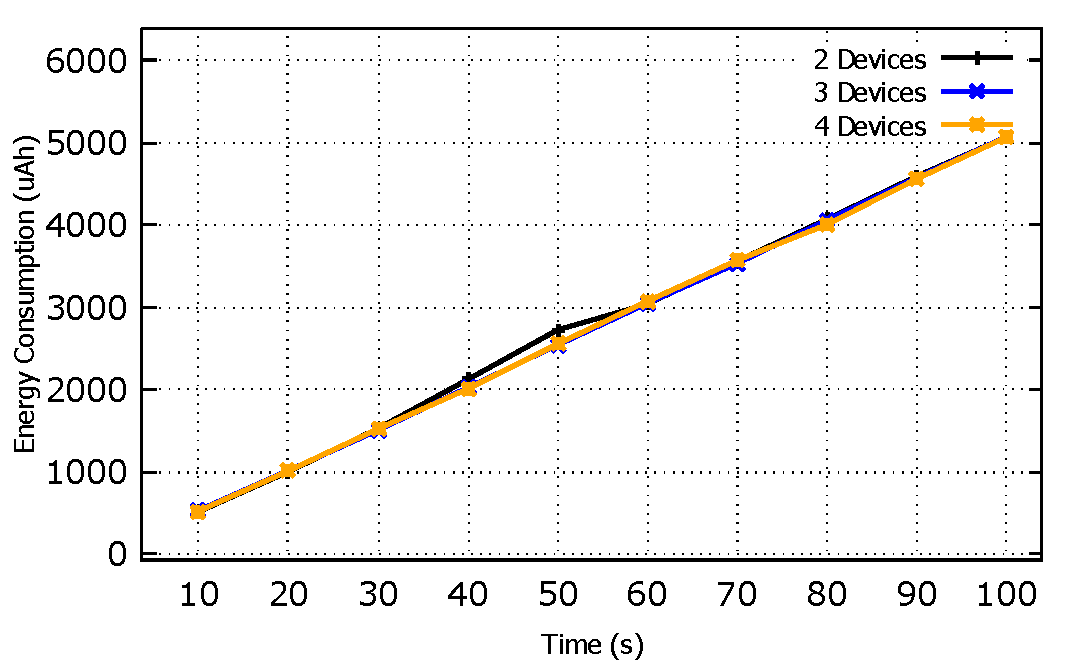
\includegraphics{data/ovh.pdf}
	}
	\caption{Total energy consumption on the caller side.}
	\label{fig:microb_24}
\end{figure}


\subsection{API Usage Scenario}
\label{sec:apiusage}
Next, we present how one can implement a mobile application using the provided programming model.

\textbf{\emph{Job Definition:}} As discussed in Section \ref{prog_model}, the programmer must define what he/she will execute remotely by overriding \texttt{exec()} of the \texttt{Job} class. Then, the provided \texttt{DexCreator} tool compiles and compacts it into the DEX jar package, which will be sent to peers or an offloading server. 


%Also, to support dynamic class loading in Dalvik VM, we provide the \texttt{DexCreator} commandline tool that compiles the \texttt{Job} Java class file into a Dex package. The Dex package and sliced resources are packed as a \texttt{JobData} object by \texttt{JobDispatcher} and then dispatched to the available mobile devices or the cloud-based server. Next, the recipient of the \texttt{JobData} checks a checksum field to confirm the consistency, and then deserializes the object into \texttt{Job} and resources for the execution.

\textbf{\emph{Data Parser:}} Next, the programmer needs to write the \texttt{DataParser} class, so that any uder-defined data can be processed at remote locations. The following code snippet \ref{code:get_single_part} shows how the programmer can partition an image file for his/her image processing application.

%\texttt{ExecutionHandler} is the main component which wraps up the complexity, and exposes only the necessary functions like \texttt{discoverPeers()} and \texttt{dispatchJob()}. To send ACK messages to other peers for exchanging acknowledgments and reforming network, we need to call \texttt{discoverPeers()} function on the program, which should be done as soon as the application starts.

\begin{figure} [!tbh]
\noindent \shadowbox{%
\begin{minipage}{.95\linewidth}
  \begin{lstlisting}
public Object getSinglePart(...) {
  Bitmap bmpData = (Bitmap) data;
  int pWidth = eOffset - sOffset;
  return Bitmap.createBitmap(bmpData, sOffset, 
									0, pWidth, bmpData.getHeight()); 
}
  \end{lstlisting}	
\end{minipage}}	
  \captionof{lstlisting}{Example of \texttt{getSinglePart()} for Bitmap}
  \label{code:get_single_part}
\end{figure}



\begin{figure*} 
	\centering
	%\resizebox{0.39\textwidth}{!}{
	%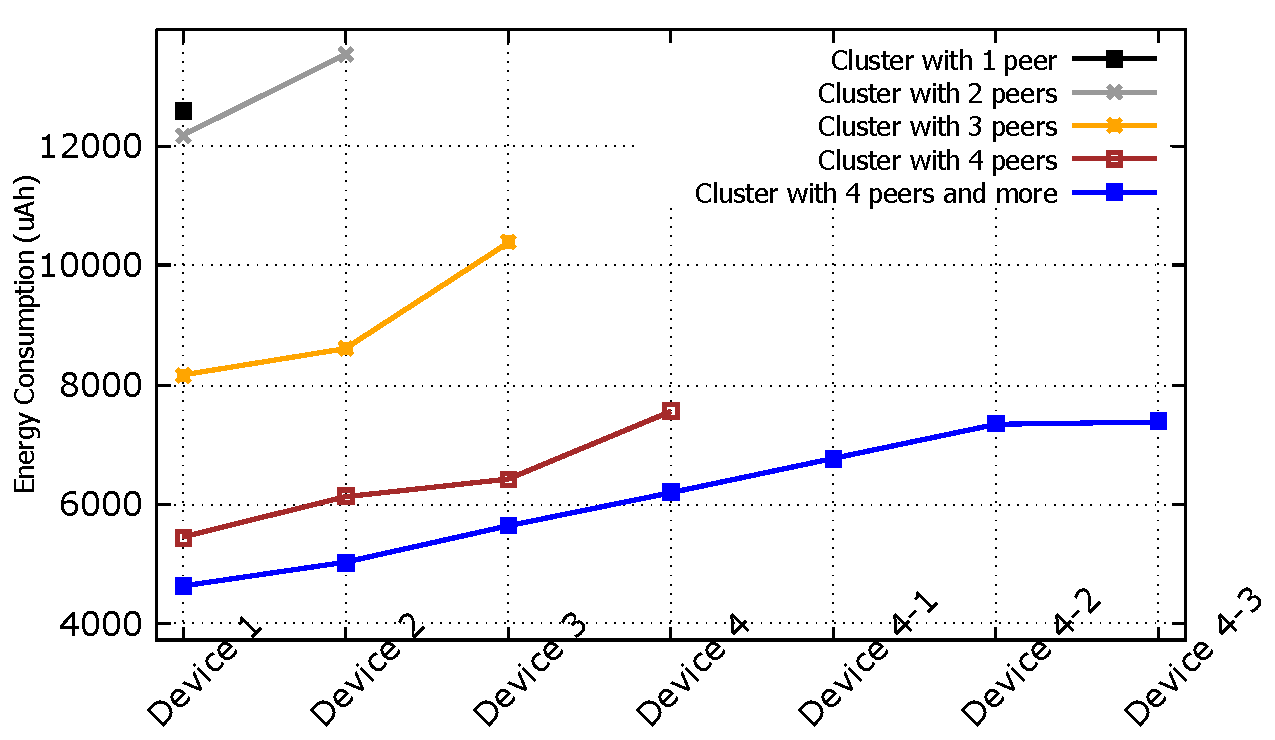
\includegraphics[width=0.32\textwidth]{data/img_large_perf_full.pdf}
		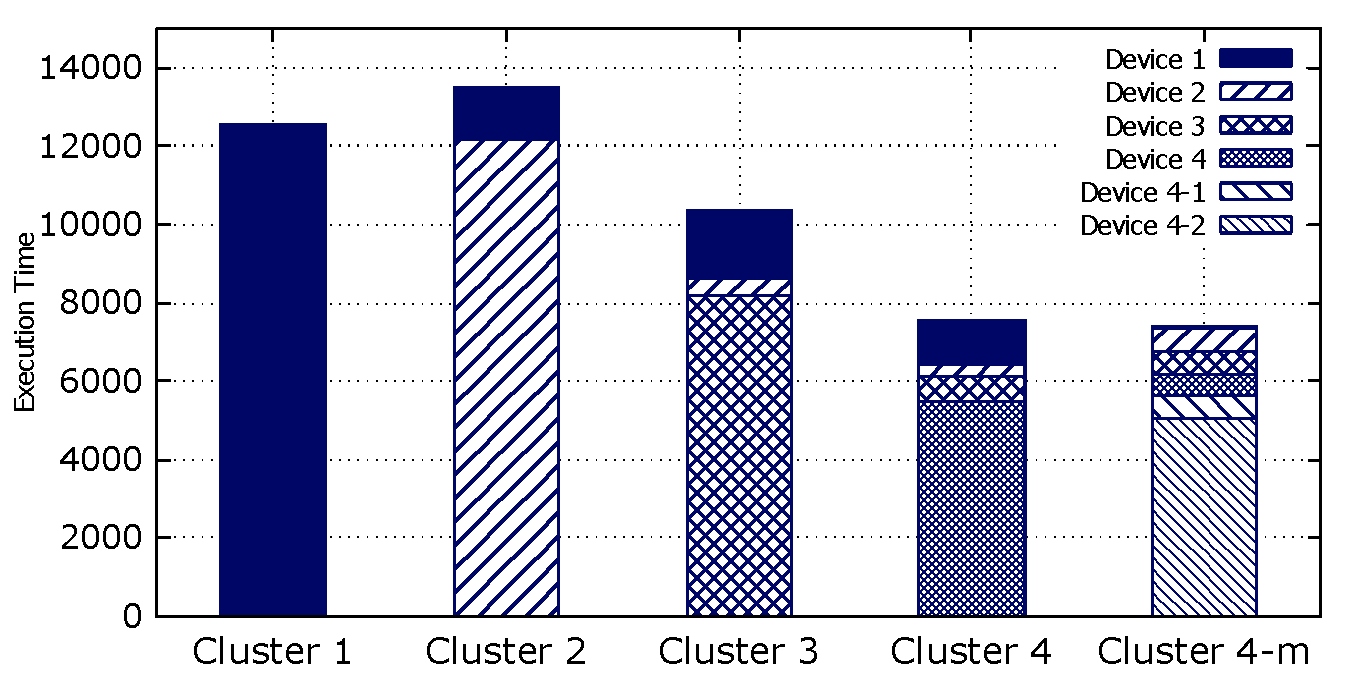
\includegraphics[width=0.45\textwidth]{data/img_perf.pdf}		
		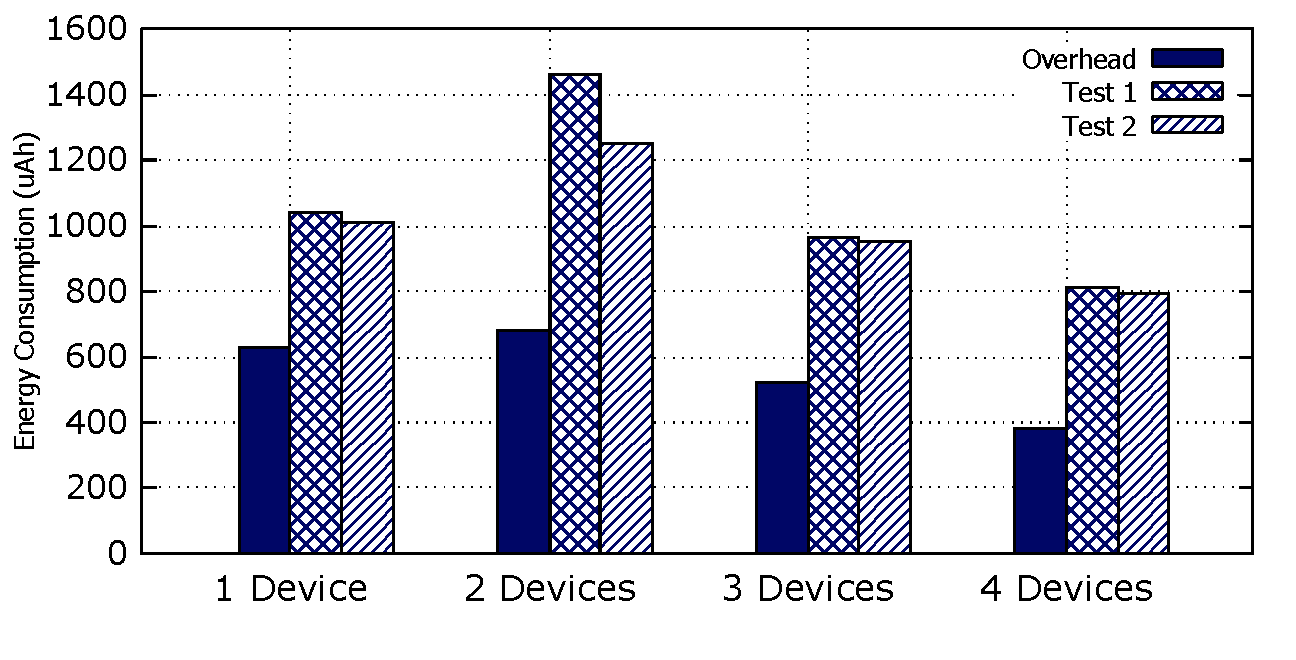
\includegraphics[width=0.45\textwidth]{data/img_energy.pdf}
	%}
	\caption{Performance and energy consumption of the large image processing tests in multiple devices.}
	\label{fig:cluster_performance}
\end{figure*}

\textbf{\emph{Message Handler:}} \emph{Message Handler} is required to be instantiated during the initialization process to receive job-related events. In Listing \ref{ui_handler}, we created \texttt{UIHandler} which handles two events---\texttt{MAIN\_INFO} containing job-related information and \texttt{MAIN\_JOB\_DONE} containing job results. 

\begin{figure} [!tbh]
\noindent \shadowbox{%
\begin{minipage}{.95\linewidth}
	\begin{lstlisting}
Handler UIHandler = new Handler() {
	public void handleMessage(Message msg) {
		switch (msg.what) {
			case Utils.MAIN_JOB_DONE: { ... }
			case Utils.MAIN_INFO: { ... } }	} };
	\end{lstlisting}
\end{minipage}
}
\captionof{lstlisting}{Message handler implementation.}
\label{ui_handler}
\end{figure}

%\textbf{\emph{Discovering Available Peers and Dispatching Jobs.}} When the network is formed and connections are held with some other peers, \texttt{dispatchJob()} will be called to locate the resources and the job which is predefined in local storage, it then invokes \texttt{DecisionMaker} (sub section \ref{scheduling}) for job splitting and binary serialization. Finally jobs will be dispatched over the socket.

%\begin{figure}
%\noindent \shadowbox{%
%\begin{minipage}{245pt}
	%\begin{lstlisting}
%dataParser = new BitmapJobDataParser();
%jobHandler = new JobHandler(this, dataParser);
%
%jobHandler.setSocketListener(
	%new JobHandler.JobSocketListener() {
		%@Override
		%public void socketUpdated(... isConnected){
			%...
		%}});
%deviceList.setAdapter(jobHandler.getDeviceListAdapter());
%jobHandler.discoverPeers();
%
%String dataPath = downloadPath + "/mars.jpg";
%String jobPath = downloadPath + "/Job.jar";
%jobHandler.dispatchJob(dataPath, jobPath);
%\end{lstlisting}
%\end{minipage}}
%
%\captionof{lstlisting}{Using DataParser and JobHandler}
%\end{figure}

\subsection{Case Study}
To measure the performance of the system equipped with our APIs, we experimented with 4 case studies using five different Android devices and 1 offloading server at an emulated testbed:
\begin{itemize} \denseitems
	\item \textbf{Image Processing:} In this case study, we initiated a P2P network to blur a large size image, which could not be loaded and processed on any single mobile device due to the limited memory space in mobile devices. Then, we distributed the blurring job to one to four mobile devices. 
	%Particularly, to process an image with size $4000 \times 4000$ and 4 bytes to express each pixel color, application must spare the amount of memory equivalent to 64MB which is way too much for a device, which occasionally returns out of memory exception.
	\item \textbf{Internet Access:} In this case study, we defined an Internet access request job for a mobile device that has limited/intermittent Internet connections, so that mobile applications could download remote data.
	\item \textbf{GPS Sharing:} Because establishing a GPS connection is a highly energy-intensive operation, it would be impossible for a device with low battery to frequently update its location information. We built a simple application that can benefit GPS locations from healthier devices. In addition, our system can be used for Internet of Things devices that do not have GPS sensors.
	\item \textbf{Using Offloading Server:} By installing Android x86 platform on a PC server, we can turn the server into a powerful and power-wired Android device and run our middleware on it without any modification.
\end{itemize}


\subsubsection{Image Processing}
We applied the blur effect, one of the high energy consuming image processes. We ran the test repeatedly with two images that have different sizes: the big image has size $4326 \times 2856$ and the smaller one has size $2500 \times 1405$. For the big one, with 4 bytes allocated for each pixel, the device had to allocate around $50MB$ of the heap to open and another $50MB$ to hold the result, thus leading to app crashes every time. This overload problem will only be solved with the help of other collaborative peers.

\begin{figure*}
	\centering
	%\resizebox{0.45\textwidth}{!}{
		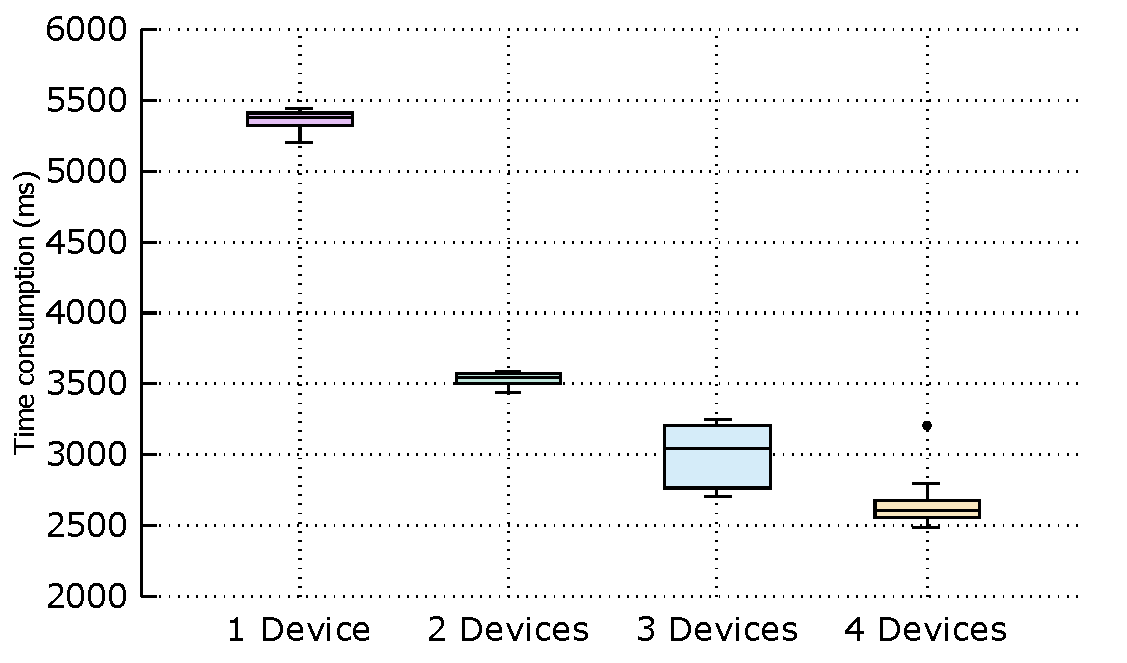
\includegraphics[width=0.48\textwidth]{data/img_small_perf_full.pdf}
		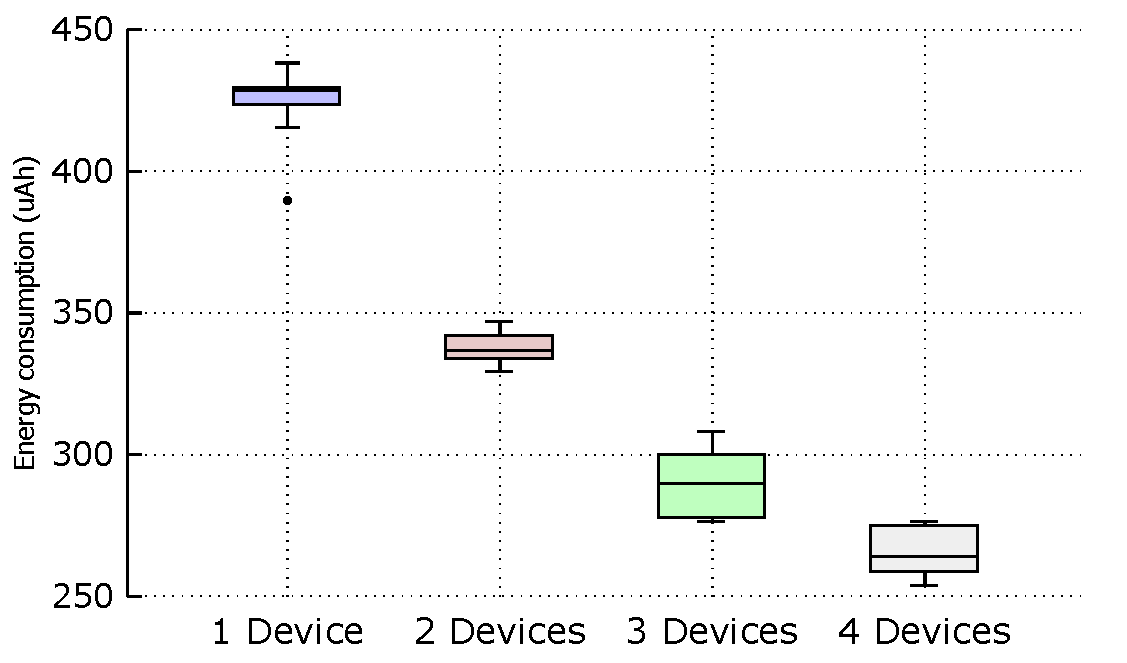
\includegraphics[width=0.45\textwidth]{data/img_small_energy.pdf}
	%}
	\caption{Performance and energy consumption of the image processing tests with a normal image size.}
	\label{fig:small_img_perf}
\end{figure*}


\textbf{\emph{Design:}}
The most important part when implementing the image processing app using the provided APIs is to define the \texttt{DataParser} (see Listing \ref{code:job_def}) for an image. In this case study, since we blur a bitmap image file, a bitmap image can be easily partitioned into small bitmap images by the \texttt{DataParser}. However, if target image files are compressed as the jpg, gif, or png format, they will need additional image processing in the \texttt{DataParser} class.

%For an input image, the \texttt{firstOffset} and \texttt{lastOffset} will decide the first and last offsets of the vertical cut correspondingly throughout the width, from the top to the bottom edges. The algorithm of the vertical cut is described in Listing \ref{code:get_single_part}. Regarding the placeholder, we override the \texttt{getJsonMetadata()} method to return a simple JSON string like below:

%\noindent \shadowbox{%
%\begin{minipage}{245pt}
	%\captionof{lstlisting}{JSON for initiating placeholder}
	%\begin{lstlisting} 
	%JSON { "width": 4326, "height": 2856 } 
	%\end{lstlisting}
%\end{minipage}
%}
%
%The \texttt{createPlaceholder()} method obtains \texttt{width} and \texttt{height} from the JSON object and then initiates an empty placeholder bitmap. Finally \texttt{copyPartToPlaceholder()} method will place the partial result bitmap into its correct location on the placeholder defined by \texttt{sOffset} and \texttt{eOffset}.\\
%
%
%Once the complete bitmap data are received, the system sends the \texttt{MAIN\_JOB\_DONE} message to the UI, in which \texttt{msg.obj} contains the final bitmap.


\textbf{\emph{Performance with a large-scale image:}}
Running a large-scale image test case throughout 50 tests by increasing the number of devices from 1 to 4 within the P2P network, we found that the test case didn't work if only one device executed desolately. By splitting the image process into two threads, we realized that only 1 thread worked, the other could not due to out of memory exception. 

By increasing the number of devices in P2P network from 2 to 4 and sending image processing jobs to the other peers, we gathered average statistic data in 20 tests as in the Figure (\ref{fig:cluster_performance} - left) (groups of 2, 3 and 4 peers). In this Figure, to accomplish the task, the two peers have to work in $13,541ms$ average. The execution time reduced when more peers participated the group, down to $7387ms$ average when 4 peers joined the group, which is twice as fast as having 2 peers (notice that system didn't fully work with only one device).

To measure energy consumption on each peer, we used Monsoon Power Monitor \cite{moosoon} to measure the velocity of energy drained on the calling device when utilizing power from the other peers. Figure \ref{fig:cluster_performance} (right) shows the energy consumption measurements from the two consecutive tests. The graph shows that the variability of energy consumption between the clusters of 2, 3 and 4 peers matches with the time consumption graph. By running the test with the same input for 20 times, we realized that the results didn't change. Also, by adding more than 3 peers, we can significantly reduce energy consumption for the image processing task to up to 25\%. However, we realized that the performance didn't significantly increase when 6 or more peers participating network. This can be explained by Amdahl's law \cite{amdahl}. Through our experiments, the number of peers at 3 to 5 will maximize the benefit in terms of energy saving and performance.

\textbf{\emph{Performance with a normal-scale image:}}
We performed the image processing test on the input image with size $2500 \times 1405$. By reconfiguring the clusters with the number of peers from 1 to 4, and measure total execution time on the caller, we gathered performance report as shown in the Figure \ref{fig:small_img_perf}. From our statistic data, the total time consumed by one device to run on itself is slightly fluctuated around $5400ms$ between 20 measurements. If one more peer joined the network, the time consumption is decreased to $3500ms$ which is 35\% faster. When more peers (3 or 4) participated, the performance of the caller will continuously increase, although their finishing time largely varied. Specifically the cluster with four peers collaboratively executed twice as fast as one device.

Essentially the variability and fluctuation of energy consumption will reflect the performance (time consumption), Figure (\ref{fig:small_img_perf} - right) displays the details. Through our experiments, running the cluster with 2 peers will preserve 20\% energy compare with 1 device, the efficiency increased in cluster with 3 peers ($34\%$) and 4 peers ($37.5\%$).

%\begin{figure}
	%\centering
	%\resizebox{0.39\textwidth}{!}{
		%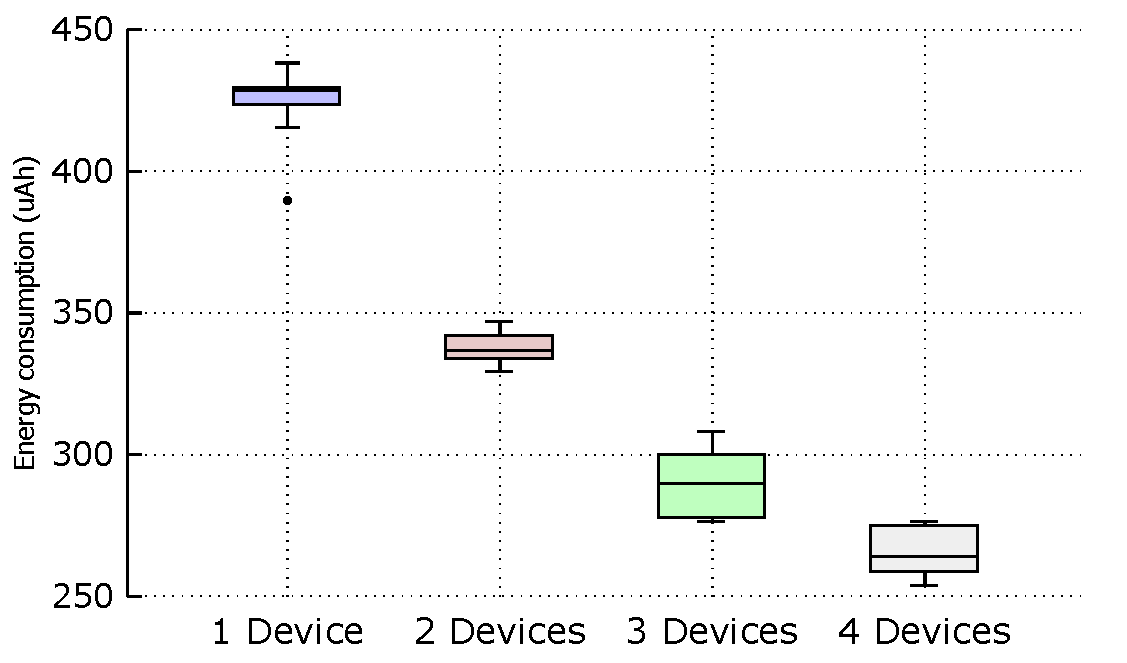
\includegraphics{data/img_small_energy.pdf}
	%}
	%\caption{Energy consumption from the image processing tests in multiple clusters.}
	%\label{fig:small_img_energy}
%\end{figure}

\subsubsection{Internet Access} 
Theoretically, remote accessibility won't help reduce the number of bytes downloaded, however, the speed is ameliorated since the downloading process is scattered over a number of peers. Thus, less energy will be consumed. 

\textbf{\emph{Design:}}
For this case study, we defined job business is to download content from a URL, and the job content will comprise of three objects: URL, the number of parts and index of the part. We also defined the initial criteria to select only the peers having Internet connection (\texttt{IRS[network]} at \texttt{high} or \texttt{low}). Once remote peers receive a job request message, their \texttt{Execution Manager} module executes the job that loads the URL and archives HTML pages locally. 

As discussed in Section Section \ref{prog_model}, to process the downloaded files including multimedia links (images, audio, videos), CSS, and JS, the programmer must implement the \texttt{DataParser} interface.Thus, our \texttt{NetDataParser} class packs all the downloaded files into one single file, which is sent back to the caller. Finally, these HTML files are opened by the Android Web browser component using a local web server, for instance, NanoHttpd \cite{nanohttpd}.

\textbf{\emph{Performance:}}
Figure (\ref{fig:net_clusters_perf} - left) describes the performance of the clusters with the number of peers varied from one to four when rendering URLs from the CNN website. At one pile, each area describes the execution time of each corresponding peer, and the pile peak is reached when the last peer has completed its job. Executing Internet access remotely through a P2P network brings a high benefit in terms of performance. For example, rendering time can be reduced by almost a half when three peers participated in the network. 


\begin{figure*}
	\centering
	%\resizebox{0.45\textwidth}{!}{
		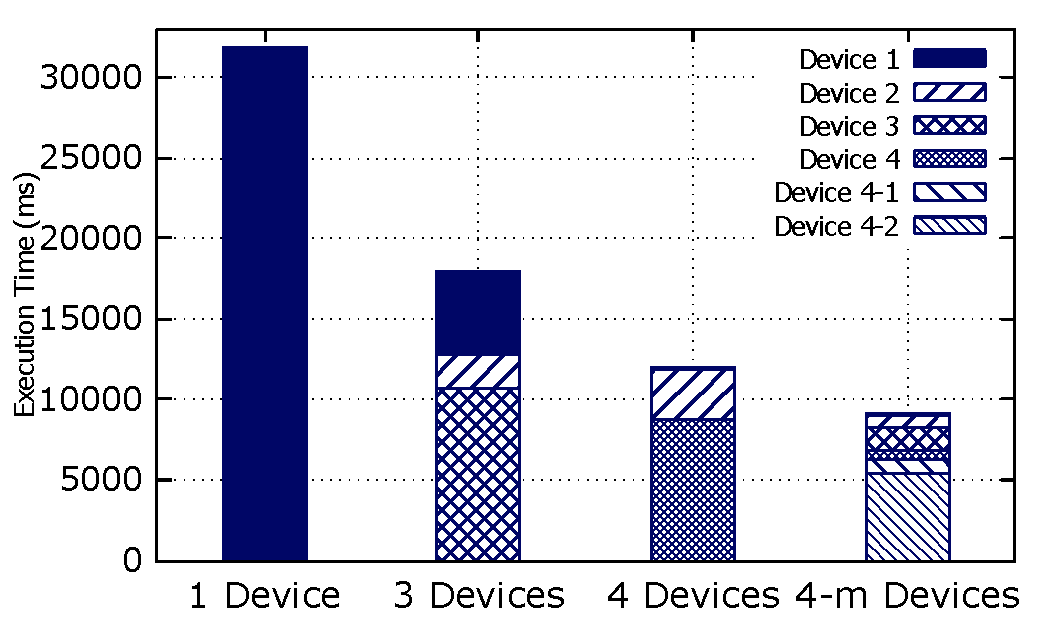
\includegraphics[width=.43\textwidth]{data/net_perf_01.pdf}
		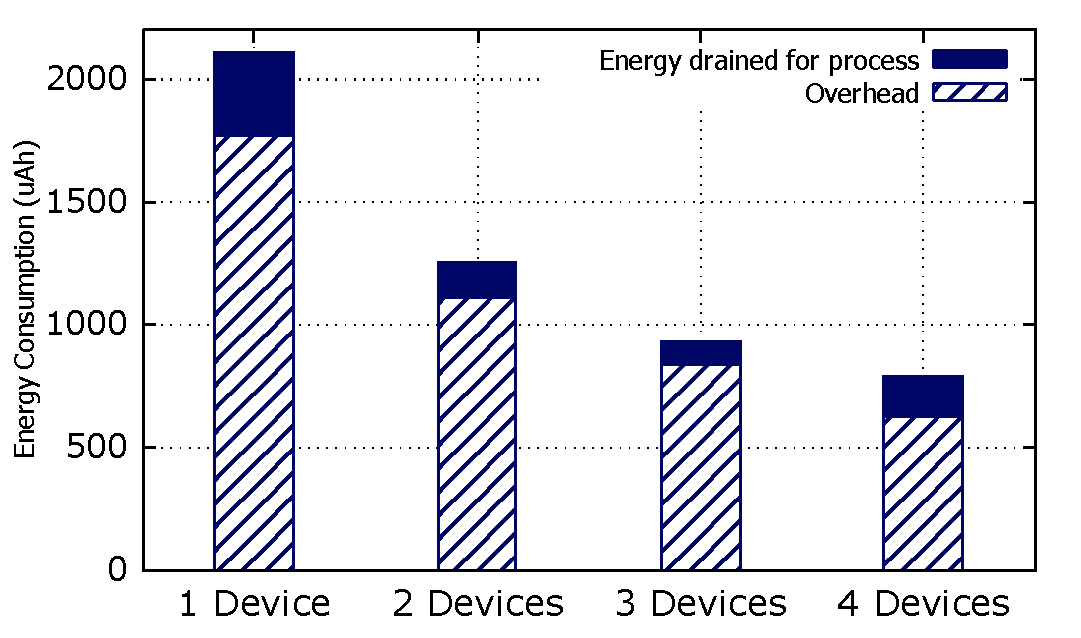
\includegraphics[width=.46\textwidth]{data/net_energy.pdf}
	%}
	\caption{Performance and energy consumption comparison for Internet sharing}
	\label{fig:net_clusters_perf}
\end{figure*}

Figure \ref{fig:net_clusters_perf} (right) depicts the outcome of the energy test. In the cluster with more than 3 peers, the energy consumption remarkably decreased up to 50\% in compare with the 1-peer cluster.

\subsubsection{GPS Sharing}
Connecting and retrieving the GPS location is really energy consuming. Generally the smartphone will enable and contact at least 3 satellites through radio signals in order to start retrieving the GPS location (4 satellites to get more information like altitude). Therefore, energy can be saved if GPS requests are relayed to another peer in P2P network, which is healthier (less battery usage or CPU is in idle state) or has better specifications.

\textbf{\emph{Design:}}
With GPS Share, only one peer is entrusted. Our strategy is letting the caller to select the peer having GPS enabled and largest value of $RL$ by configuring the caller with initiative criteria comprise of \texttt{max} $RL$ and \texttt{GPS} is \texttt{on}. Regarding job definition, we utilize the \texttt{LocationManager} object from the Android SDK to retrieve one single location result per each request and store the result to a simple string. For remote GPS request, we have to avoid callback function calls from \texttt{LocationManager}; therefore, retrieving multiple requests periodically is not effective.


\textbf{\emph{Performance:}}
We experimented with three GPS test cases: 2 for remote GPS requests and 1 for local GPS (Using GPS by itself). For each case we execute $10$ times on two devices with the same specifications and assign roles to them as a caller and a receiver to minimize the overloads throughout the system. Figure \ref{fig:gps_perf} interprets that GPS Share mechanism doesn't give any benefit in terms of performance, since the remote device has the same resource specs and remote GPS may require even more time including time for GPS location request, plus time for data transmission back to the caller (however it is too short for the consideration).

Figure \ref{fig:gps_perf} describes the distribution of energy consumptions among the 3 test cases. By applying interpolation to find trend lines for these energy distributions, we got $y = 0.053 \times x + 7.32$ formula for test 1 (Remote GPS), $y = 0.055 \times x + 7.42$ for test 2 (Remote GPS) and $y = 0.057 \times x - 12.94$ for test 3 (Local GPS). Since the trend line 3 has the biggest slope, it refers that at the same running time, it consumed more energy than the others. As we might see, the difference between the slopes of line 3 and line 1, 2 is very slim, but due to our later tests on the weak caller (with low battery), the difference will highly increase. 

\textbf{\emph{Applications:}}
By integrating our system with either RetroSkeleton \cite{retro-skel} or Rio \cite{rio}, we can extend GPS location requests to the other nearby devices without any modification to the existing applications. Those systems provide interference methods to capture requests for system resources and instead inject their custom responses. 

\begin{figure*}
	\centering
	%\resizebox{0.36\textwidth}{!}{
		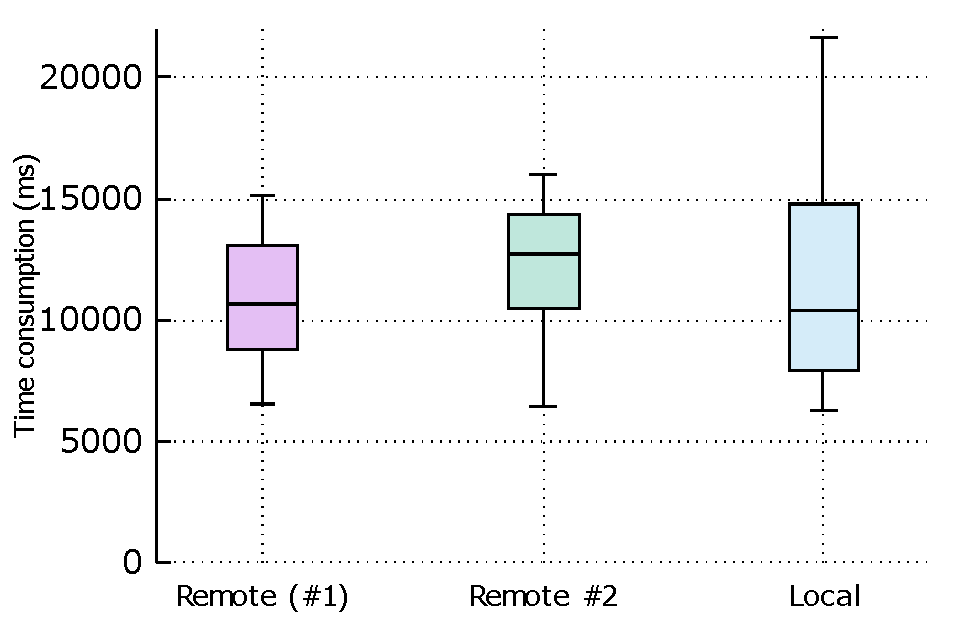
\includegraphics[width=.42\textwidth]{data/gps_perf.pdf}
		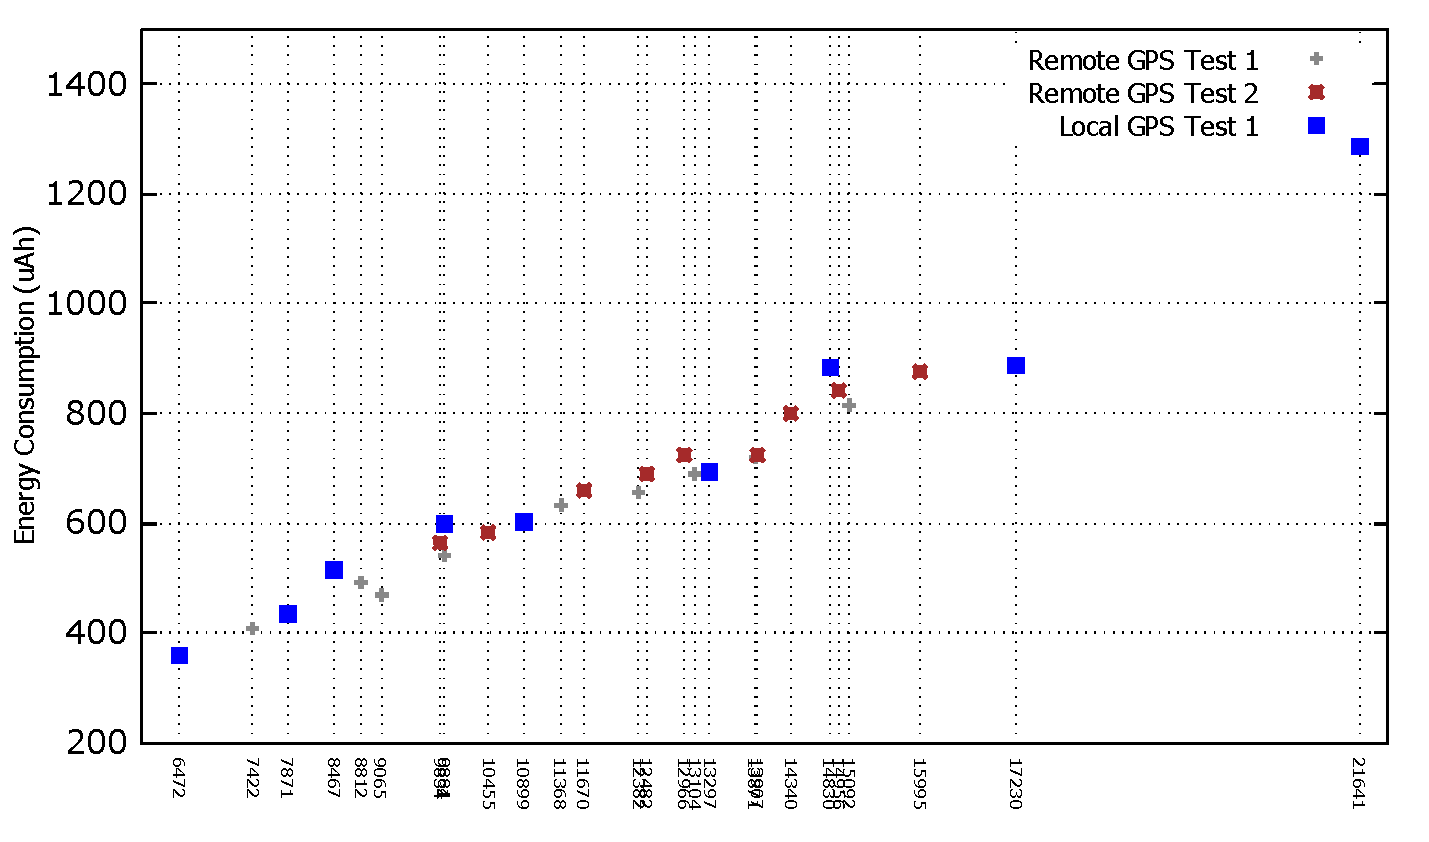
\includegraphics[width=.47\textwidth]{data/gps_energy_full.pdf}
	%}
	\caption{Performance and energy consumption comparison between remote and local GPS sensing.}
	\label{fig:gps_perf}
\end{figure*}

\subsubsection{With Offloading Server}
Lastly, we compare peer to peer- and offloading server-based executions regarding performance and energy efficiency.

\textbf{\emph{Experimental Setup:}}
For an offloading server, we installed Android x86 platform on a PC, so that we could host our implementations without any modification. Only the server address was configured in advance. 

If a caller determines that executing a job on the offloading server is more beneficial than running through nearby devices, it will connect to the server and disconnects the communication channels established with the other peers. Then, the runtime system offloads the whole job to the server with data. One copy of the job will be maintained at the caller for handling faults.

To emulate different networks (LAN, WLAN and WAN), we have used \texttt{Network Emulator for Windows Toolkit} \cite{newt}, a popular network emulator. Particularly, we set 0ms latency for LAN, 50ms for WLAN, and 150ms for WAN.


\textbf{\emph{Experimental Results:}}
We experimented with the image processing case study with the same small-scale image. When increasing the latencies of both incoming and out-going packages of the server network from 0 to 500ms, we observed that the time and energy consumption also steadily increased (Figure \ref{fig:off_all}). We have the following observations:
\begin{itemize} \denseitems
	\item The cloud offloading in WAN environment (i.e., limited and intermittent latency/bandwidth) has limited benefits in terms of performance and energy efficiency compared to the P2P-based offloading.
	\item The cloud offloading in WLAN environment (i.e., moderate latency/bandwidth), is sometimes more beneficial than the P2P-based offloading in terms of energy efficiency but does not have performance benefits.
	\item The cloud offloading in LAN environment (i.e., favorable latency/bandwidth)completely overwhelms the P2P-based offloading regardless of the number of peers.
\end{itemize}

As a result, we can argue that different offloading mechanisms should be selected in accordance with various network conditions (i.e., latency/bandwidth characteristics) and different jobs (i.e., computation-intensive vs. sensor-based executions) in a dynamic, adaptive way to achieve further optimizations. 
%\cite{ELI}

%When comparing with the previous results executing on a peer-to-peer network through nearby devices, 
\subsection{Threats to Validity}
The results presented above are subject to internal and external validity threats. The internal validity is threatened by how the interactive subject applications were exercised. The performance and energy consumption of interaction applications depend on how the user chooses to use them. To minimize this threat, the benchmarked use cases were fixed to using the same media (i.e., picture file), location (i.e., GPS coordinates), and Internet URL. Another internal validity threat is the fashion in which we implemented the jobs (e.g., blur effect). To minimize this menace, we took advantage of built-in Android libraries to implement these jobs.

The external validity is threatened by the mechanism to measure energy consumption. We measure the physical consumed energy directly using a power monitoring tool, which does not isolate the energy consumption of the subject applications from the total energy consumption of the whole mobile device. Thus, the energy consumption of the subject applications is subject to background services. To minimize this threat, we uninstalled all the third-party applications and stopped unnecessary background services.

\begin{figure*}
	\centering
	%\resizebox{0.36\textwidth}{!}{
		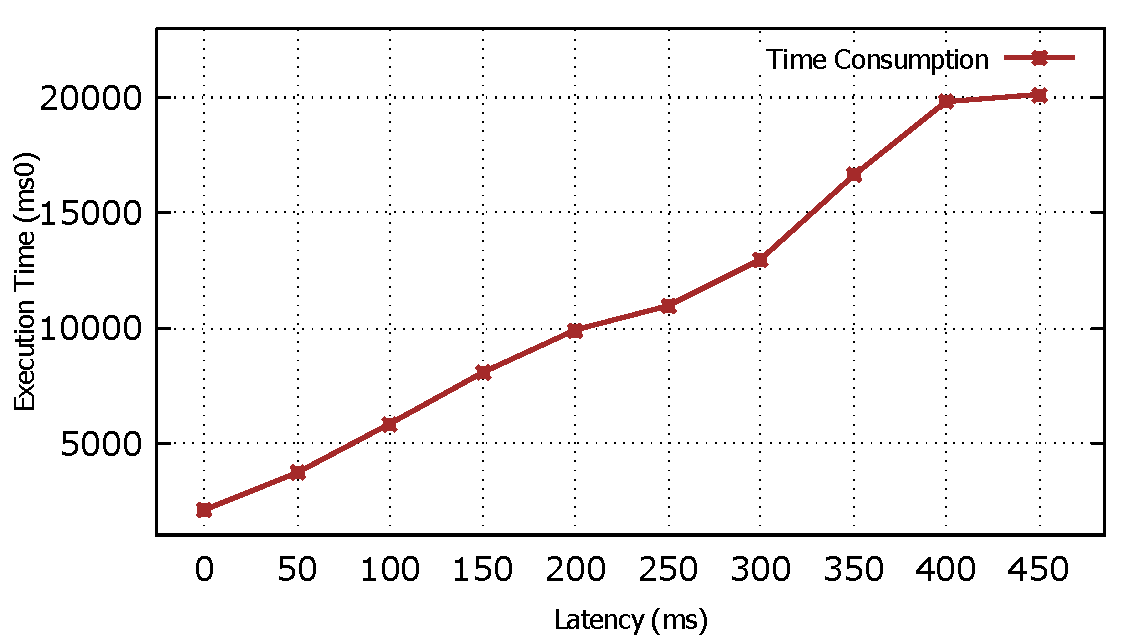
\includegraphics[width=.42\textwidth]{data/off_multi_perf.pdf}
		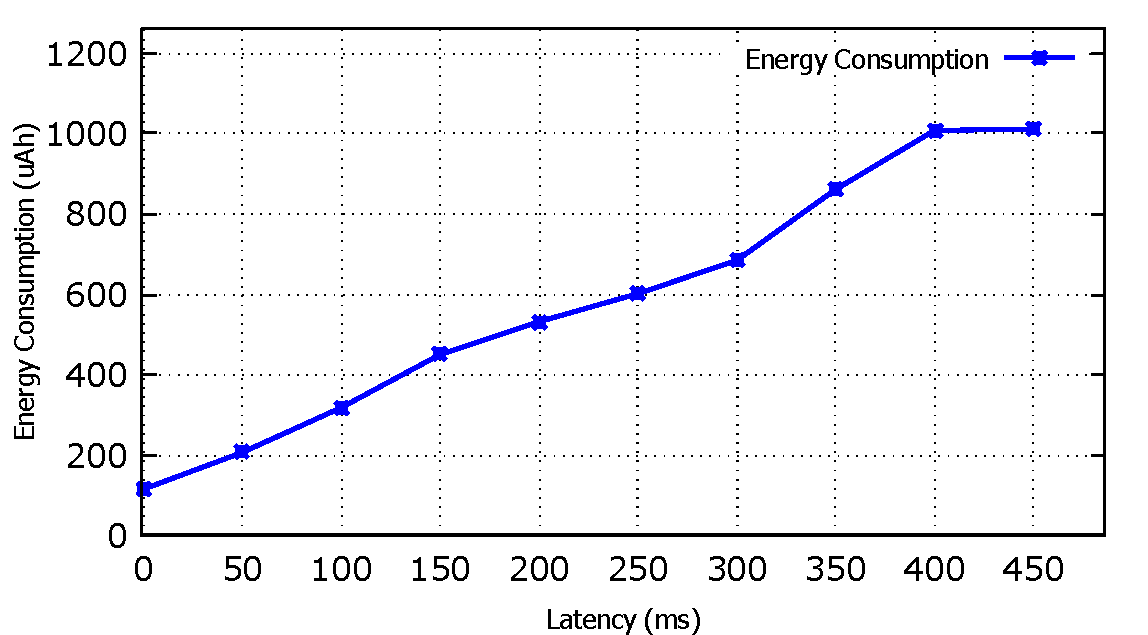
\includegraphics[width=.42\textwidth]{data/off_multi_energy.pdf}
	%}
	\caption{Performance and energy consumption comparison between remote and local GPS sensing.}
	\label{fig:off_all}
\end{figure*}

\subsection{Discussion}
Despite its benefits, one can argue that executing any class files on a mobile device is harmful in terms of privacy and security. Thus, we will make our runtime system configurable as a future research direction. The implementation will provide a configuration file that can be used to specify user preferences with respect to battery, privacy, security, etc. In particular, a configuration file contains a set of key/value pairs, with the keys of \texttt{battery\_level}, \texttt{trusted\_host}, and \texttt{privilege}, which will indicate the favorable battery level for requested job executions, trusted network or peer list, and local resource access rights (e.g., CPU, memory, local files, or sensors), respectively.

%The \texttt{trusted_host} key points to the locations of the available offloading servers. The \texttt{mode} key points to the value specifying whether the offloading should be plain (i.e., always offload the specified hotspot method) or adaptive (i.e., decide whether to offload at runtime based on the conditions in place). The \texttt{criteria} key defines which notion of \emph{effectiveness} should be used with a given offloading. The \texttt{criteria} value of \texttt{energy} indicates the effectiveness to reduce energy consumption, while that of \texttt{performance} to speed up performance. The value of \texttt{epr} indicates the effectiveness to increase the energy/performance ratio that correlates performance and energy consumption values so as to maximize the resulting correlation. The \texttt{strategy} key points to well-known energy optimization techniques, including data compression, reducing image quality, and redirecting to an easier-to-reach remote server. 

%Another limitation of our approach is 
%\subsubsection{Security}

\section{Related Work}
\label{sec:related}
The work presented here is related to other complementary efforts that optimize mobile applications' performance and energy efficiency via remote executions including software library for developers, peer to peer networking, code migration and computation offloading.

Alljoyn \cite{alljoyn} is an open source framework that hides the complexity of network communications for application programmers. By providing interoperability between multiple platforms without any transport layers, Alljoyn makes the integration and initiation of network communication easy and straightforward. Before the Wi-Fi Direct technology, many efforts have spent to address peer-to-peer network based on existing short-range/wireless communication technologies available on mobile devices including Bluetooth, Wireless IEEE802.11 and cellular communication link \cite{m_p2p_tutor,bella+:context_aware_mid}. 

In the category of Wireless-based peer-to-peer communication, before the Wi-Fi Direct technology, there have been several researches utilizing other wireless communications to establish P2P network such as media sharing system in urban transport using Bluetooth \cite{media_share}, resource sharing using cellular networks \cite{chia+:res_share}, radio resource sharing over ultra-wideband \cite{cuomo+:radio_share}. Built on top of Wi-Fi P2P, Rio \cite{rio} leverage I/O system devices to capture and share contents and resources between the existing applications running on different devices without any modification. Some of their applications are multi-system photography and gaming, singular SIM card for multi-devices, music and video sharing. GameOn \cite{gameon} also built on the same network infrastructure to establish non-Internet connection between gamers within closed range networks like in public transportation. CAMEO \cite{cameo}, and GigaSight \cite{crowd-sourcing} are also the similar content sharing systems in closed range network architecture.


%Spartacus \cite{spartacus} introduced a new communication method called spatially-aware neighboring device interactions using the Doppler sound effect to trigger the gesture detection service. The experimental results show the selection accuracy up to 90\% within 3 meters and more efficient than WiFi and Bluetooth in terms of energy consumption.

Another relevant work to our approach is one that migrates different code bases into a system. In particular, code migration can be used to update existing, legacy systems \cite{Emmerich:2000:IIC:337180.337227}. Similar to our approach, code migration mechanisms are mainly used to run code on different memory spaces (e.g., running C++ code on multi-core systems \cite{Cooper:2010:OAC:2174824.2174856}, running JavaScript code on a server \cite{Tseng:2015:MJM:2695664.2695987}, object-level migration for distributed systems \cite{Yoshida:2007:CMC:1378063.1378069}, thread-level migration through middleware \cite{Truyen:2000:PST:647629.732581}). These code migration works also have affected the execution offloading mechanisms in the mobile computing area. Thus, we compare our work with several well-known offloading approaches in the following discussion.

Finally, our work shares objectives and techniques with execution  offloading approaches \cite{maui,comet,mobile-cloud-middleware,fuzzy-engine,sokol+:thinkair}. These offloading mechanisms is a well-known mobile application optimization technique that makes it possible to execute the application's energy intensive functionality at a powerful cloud-based server, without draining the mobile device's battery. In this paper, we have focused on generalizing these offloading mechanisms using two different distributed execution models---client/server and peer to peer communication models. In addition, we enabled resource-limited devices to expand their hardware capacities through various distributed execution modles.


\begin{figure*}
\centering
	%\resizebox{0.36\textwidth}{!}{
		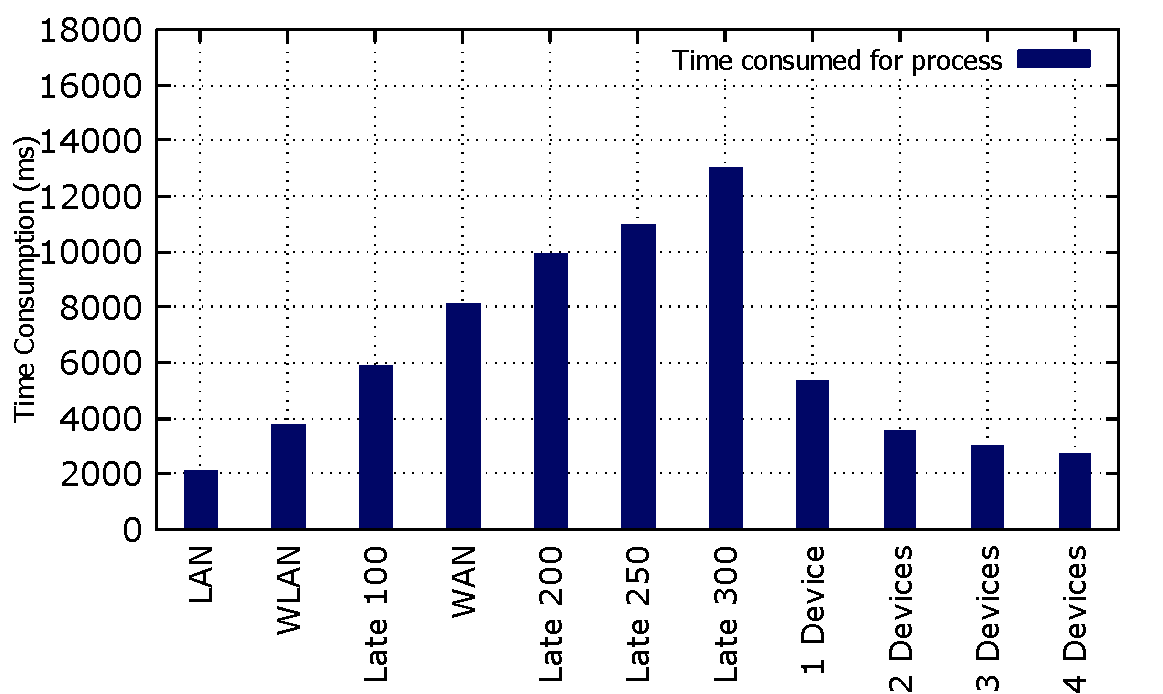
\includegraphics[width=.42\textwidth]{data/off_compare_img_perf.pdf}
		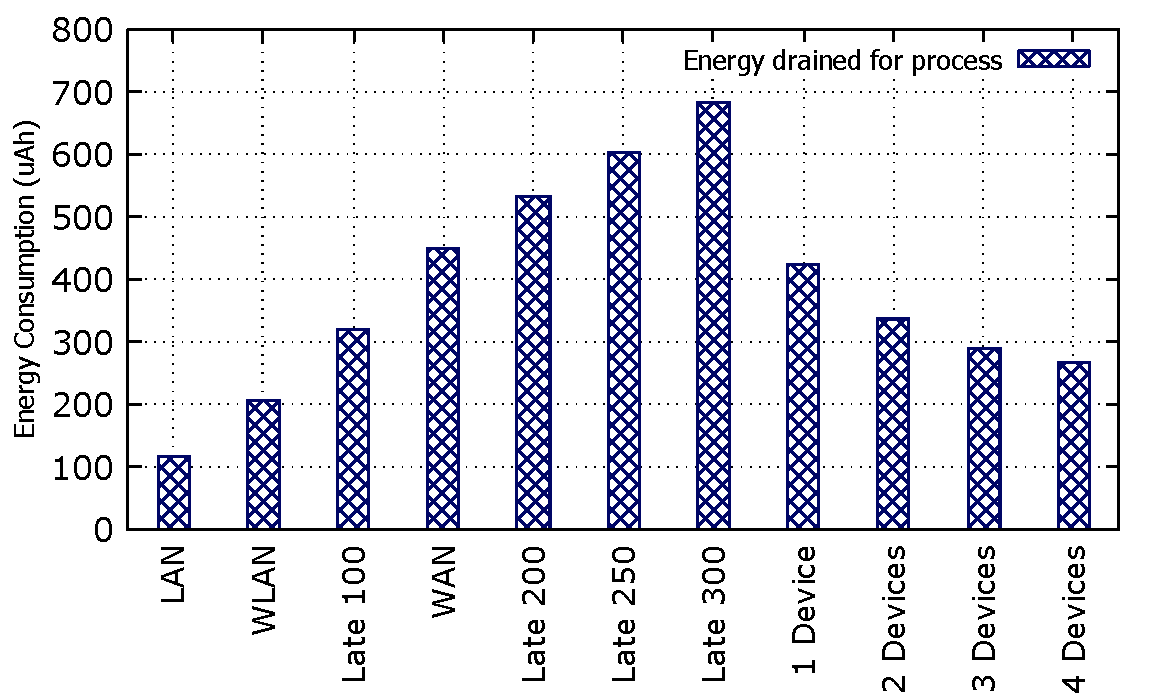
\includegraphics[width=.42\textwidth]{data/off_compare_img_energy.pdf}
	%}
	\caption{Experimental results of the Image processing when using the cloud offloading.}
	\label{fig:off_compare_img}
\end{figure*}


\section{Conclusions}
\label{sec:conc}
%Our future research direction will 
%
In this paper, we have presented an extended distribution framework to increase the quality of service in resources-limited execution environments. Our approach improves the energy efficiency and performance of mobile applications with a simple programming model and a novel runtime system by leveraging either cloud infrastructures or nearby mobile devices. In addition, our approach can bring a new hardware feature to the existing mobile devices. We have evaluated our approach by reducing the execution time and the energy consumption of case study applications as well as enabling a mobile device to utilize a GPS sensor from nearby mobile devices. These results indicate that our approach represents a promising direction in developing complex mobile applications for resource-limited mobile devices.

%\section*{Acknowledgment}
%This research is supported by Utah State University through the RC Grant.

\balance
\bibliographystyle{abbrv}
\bibliography{references}

\end{document}

